% !TeX root = bagrut-all.tex
	
\selectlanguage{hebrew}

\chapter{חדו"א שאלה 
$7$}

%%%%%%%%%%%%%%%%%%%%%%%%%%%%%%%%%%%%%%%%%%%%%%%%%%%%%%%%%%%%%%%%%%%%%%

\section{קיץ תשע"ח מועד ב}

\begin{center}
\selectlanguage{english}
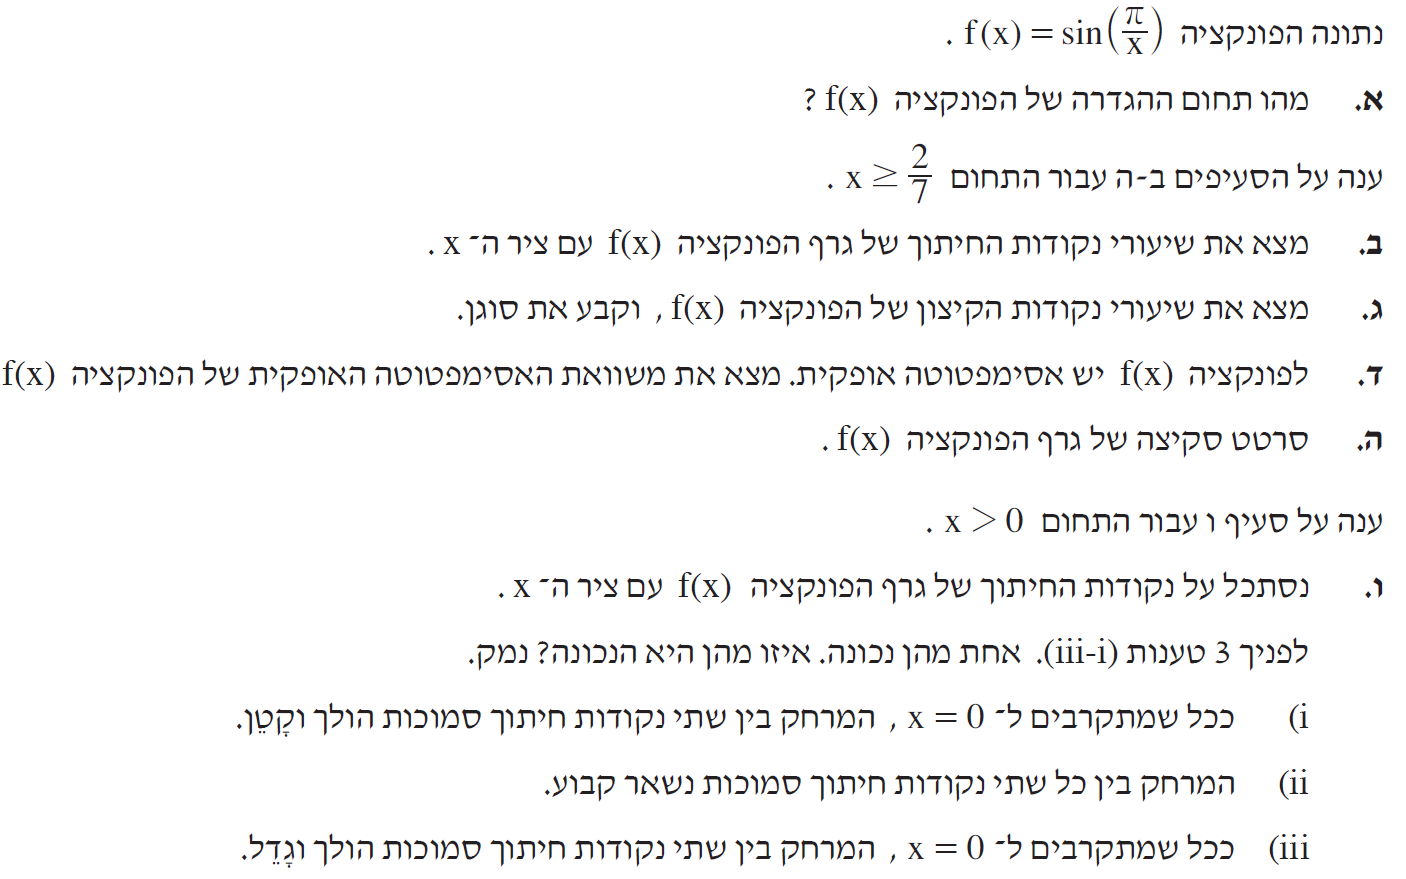
\includegraphics[width=\textwidth]{summer-2018b-7}
\end{center}

\vspace{-2ex}

\textbf{סעיף א}

הפונקציה מוגדרת כאשר במכנה 
$x\neq 0$.

\smallskip

\textbf{סעיף ב}
\[
\sin\left(\frac{\pi}{x}\right)=0,\quad\quad \frac{\pi}{x}=k\pi,\quad\quad x=\frac{1}{k}\,.
\]
נבדוק עבור כמה ערכים של
$[k,x]$:
\[
[1,1],\;\left[2,\frac{1}{2}\right],\;\left[3,\frac{1}{3}\right],\;\left[4,\frac{1}{4}\right]\,.
\]
אבל
$\disfrac{2}{7}\approx 0.286$
כך שעבור
$k\geq 4$,
הנקודות מחוץ לתחום. נקודות החיתוך הן:
\[
\left(\frac{1}{3},0\right),\; \left(\frac{1}{2},0\right), \; (1,0)\,.
\]

\vspace{-3ex}

\textbf{סעיף ג}
\[
\left(\sin\left(\frac{\pi}{x}\right)\right)'=\cos\left(\frac{\pi}{x}\right)\cdot \left(-\frac{\pi}{x^2}\right)=0\,.
\]
הגורם
$-\disfrac{\pi}{x^2}$
לא יכול לקבל ערך אפס, ולכן נקודות הקיצון הן הנקודות:
\[
\frac{\pi}{x}=\frac{\pi}{2}+k\pi,\quad\quad \frac{1}{x}=\frac{1}{2}+k,\quad\quad x=\frac{2}{1+2k}\,.
\]

\np

נבדוק עבור כמה ערכים של
$[k,x]$:
\[
[0,2],\;\left[1,\frac{2}{3}\right],\;\left[2,\frac{2}{5}\right],\;\left[3,\frac{2}{7}\right]\,.
\]
ברור שעבור 
$k\geq 4$
הנקודות מחוץ לתחום.

לפי הערכים של
$f(x)$
אפשר לקבוע את סוג נקודות הקיצון:
\[
\left(\frac{2}{7},-1\right)\;\textrm{\R{מינימום}}\quad
\left(\frac{2}{5},1\right)\;\textrm{\R{מקסימום}}\quad
\left(\frac{2}{3},-1\right)\;\textrm{\R{מינימום}}\quad
(2,1)\;\textrm{\R{מקסימום}}
\]
אפשר לבדוק לפי נגזרת שנייה. המכנה של הנגזרת הראשונה
$x^2$
חיובית, ולכן מספיק לבדוק את הסימן של הנגזרת של המונה:
\[
-\left(\cos \left(\frac{\pi}{x}\right)\right)'=-\left(-\sin\left(\frac{\pi}{x}\right)\right)\cdot \left(-\frac{\pi}{x^2}\right)=-\frac{\pi}{x^2}\cdot\sin\left(\frac{\pi}{x}\right)\,.
\]
מכאן שסימן הנגזרת השנייה תלוי בסימן של
$-\sin\left(\frac{\pi}{x}\right)$.
\[
-\sin\left(\frac{\pi}{2}\right)=-1,\quad
-\sin\left(\frac{3\pi}{2}\right)=1,\quad
-\sin\left(\frac{5\pi}{2}\right)=-1,\quad
-\sin\left(\frac{7\pi}{2}\right)=1\,.
\]
הסימנים תואמים את קביעת סוג נקודות הקיצון שרשמנו.

\textbf{סעיף ד}

$\disfrac{\pi}{x} \limit{+\infty} 0$
ו-%
$f(x)=\sin\left(\disfrac{\pi}{x}\right)\limit{+\infty} 0$.
יש
\asm{}
אופקית ב-%
$y=0$.

\textbf{סעיף ה}

נקודות הקיצון מסומנות:
\begin{center}
\selectlanguage{english}
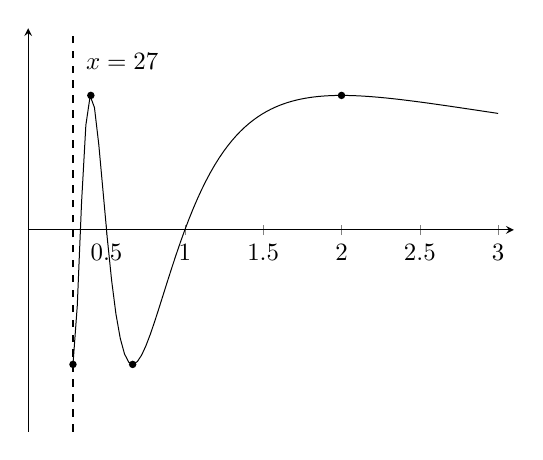
\begin{tikzpicture}[scale=.9]
\begin{axis}[
    trig format plots=rad,
    axis lines=center,
    xmin = 0,
    xmax = 3.1,
    ymin = -1.5,
    ymax = 1.5,
    ymajorticks=false,
]
\addplot [
    domain=.286:3,
    samples=100, 
]
{sin(rad 3.14159/rad x)};
\draw[dashed,thick] (axis cs:.286,-1.5) -- (axis cs:.286,1.5);
\fill (axis cs:.286,-1) circle(1.5pt);
\fill (axis cs:.667,-1) circle(1.5pt);
\fill (axis cs:.4,1) circle(1.5pt);
\fill (axis cs:2,1) circle(1.5pt);
\node at (axis cs:.6,1.25) {$x=\disfrac{2}{7}$};
\end{axis}
\end{tikzpicture}
\end{center}

\vspace{-2ex}

\textbf{סעיף ו}

$x=\disfrac{1}{k}$.
ככל ש-%
$x$
מתקרב לאפס
$k$
עולה. המרחק בין שתי נקודות חיתוך סמוכות
$\disfrac{1}{k},\disfrac{1}{k+1}$
הוא:
\[
\frac{1}{k}-\frac{1}{k+1}=\frac{1}{k(k+1)}\,,
\]
וברור שערך זה קטן ככל ש-%
$x$
מתקרב לאפס ו-%
$k$
עולה. המסקנה היא ש-%
$(i)$
נכון.

\np


%%%%%%%%%%%%%%%%%%%%%%%%%%%%%%%%%%%%%%%%%%%%%%%%%%%%%%%%%%%%%%%%%%%%%%

\section{קיץ תשע"ח מועד א}

\begin{center}
\selectlanguage{english}
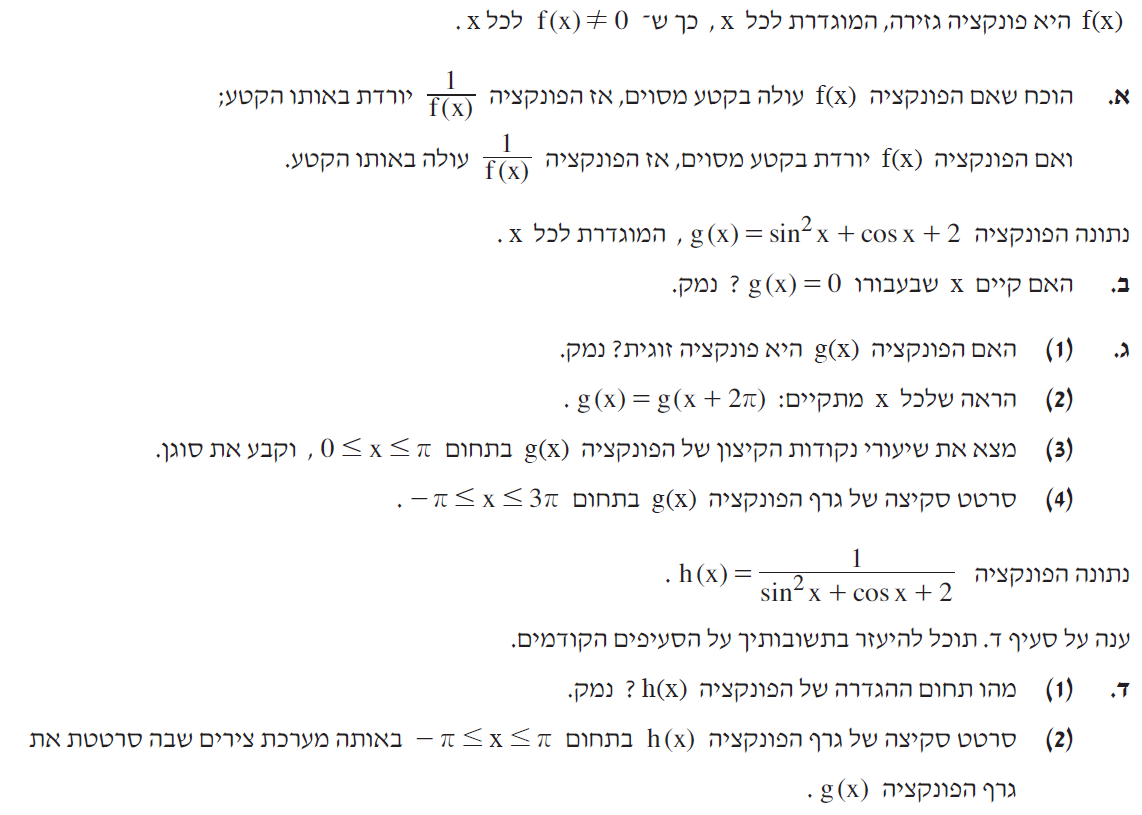
\includegraphics[width=\textwidth]{summer-2018a-7}
\end{center}

\vspace{-2ex}

\textbf{סעיף א}

לכאורה הטיעון ברור מאליו אבל כנראה שצריך להוכיח באמצעות הנגזרות:
\[
\left(\frac{1}{f(x)}\right)'=-1\cdot f(x)^{-2} \cdot f'(x)\,.
\]
נתון ש-%
$f(x)$
מוגדרת בכל התחום, ו-%
$f(x)^{-2}$
חיובי בכל התחום. הסימן של
$\left(\frac{1}{f(x)}\right)'$
הפוך מהסימן של
$f'(x)$,
ולכן אם
$f(x)$
עולה 
$\frac{1}{f(x)}$
יורדת, ולהיפך.

\medskip

\textbf{סעיף ב}

$\sin^2 x\geq 0$
ו-%
$\cos x \geq -1$.
לכן 
$g(x)= \sin^2 x + \cos x + 2 \geq 1$
והפונקציה לא מתאפסת.

\medskip

\textbf{סעיף ג}

$(1)$
הפונקציה זוגית, כי 
$\cos$
זוגית ו-%
$\sin$
אי-זוגית, אבל 
$\sin^2$
זוגית. בחישוב:
\[\sin^2 (-x)+\cos (-x)  +2=(-\sin x)^2+\cos x + 2=\sin^2 x+\cos x + 2\,.
\]

\np

$(2)$
$\sin (x+2\pi)=\sin x, \cos (x+2\pi) = \cos x$
ולכן 
$g(x)=g(x+2\pi)$.

אפשר גם לחשב:
\erh{2pt}
\begin{equationarray*}{l}
\sin^2 (x+2\pi) + \cos (x+2\pi) + 2 =\\
\hspace*{3em}(\sin x \cos 2\pi + \sin 2\pi \cos x)^2 + (\cos x \cos 2\pi - \sin  x\sin 2\pi) + 2=\\
\hspace*{3em}\sin^2 x + \cos x + 2\,.
\end{equationarray*}

\vspace{-4ex}

$(3)$
נחשב את הנגזרת הראשונה:
\[
g'(x)=2\sin x \cos x - \sin x=\sin x(2\cos x - 1) = 0\,.
\]
בתחום
$0\leq x \leq \pi$,
$\sin x$
מתאפס ב-%
$x=0, x=\pi$,
ו-%
$2\cos x-1$
מתאפס ב-%
$\disfrac{\pi}{3}$.
נקודות הקיצון הן
$(0,3),\left(\disfrac{\pi}{3},\disfrac{13}{4}\right),(\pi,1)$.
נחשב את הנגזרת השנייה:
\erh{2pt}
\begin{equationarray*}{rcl}
g''(x)&=&\cos x(2\cos x-1) + \sin x(-2\sin x)\\
&=&2\cos^2 x -2\sin^2 x - \cos x\\
&=&2\cos^2 x -2(1-\cos^2 x) - \cos x\\
&=& 4\cos^2 x -2 -\cos x\,.
\end{equationarray*}
בנקודות הקיצון:
$g''(0)=1$
והנקודה היא מינימום.
$g''\left(\frac{\pi}{3}\right)=-\frac{3}{2}$
והנקודה היא מקסימום.

$g''(\pi)=3$
והנקודה היא מינימום.

$(4)$
לפי נקודות הקיצון נצייר את הגרף עבור
$0\leq x \leq \pi$.
לפי
$(1)$
הפונקציה זוגית אז הגרף עבור
$-\pi\leq x \leq 0$
זהה. לפי
$(2)$
הפונקציה מחזורית וניתן להעתיק את הגרף לתחום
$\pi\leq x \leq 3\pi$.


\begin{center}
\selectlanguage{english}
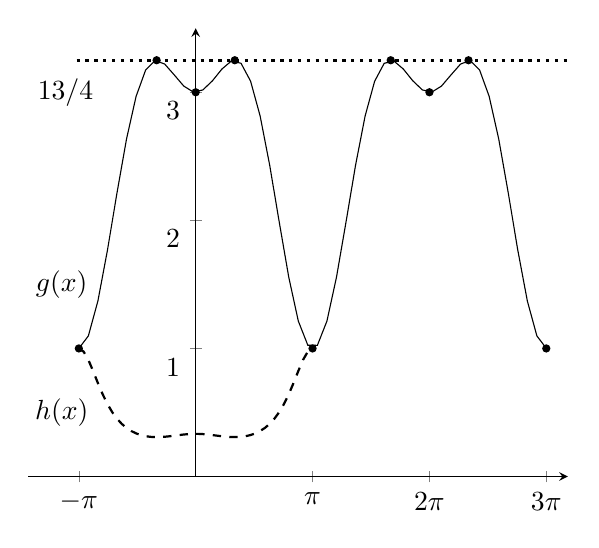
\begin{tikzpicture}%[scale=.8]
\begin{axis}[
    trig format plots=rad,
    axis lines=center,
    xmin = -4.5,
    xmax = 10,
    xtick={-3.14,0,3.14,6.28,9.42},
    xticklabels={$-\pi$,$0$, $\pi$, $2\pi$, $3\pi$},
    ymin = 0,
    ymax = 3.5,
    yticklabel style={anchor=north east},
]
\addplot [
    domain=-3.141:9.424,
    samples=50, 
]
{(sin(x))^2 + cos(x)+ 2};
\addplot [
    domain=-3.141:3.141,
    samples=50,
    thick,
    dashed,
]
{(1)/((sin(x))^2 + cos(x)+ 2)};
\fill (axis cs:-3.14,1) circle(1.5pt);
\fill (axis cs:3.14,1) circle(1.5pt);
\fill (axis cs:9.42,1) circle(1.5pt);
\fill (axis cs:0,3) circle(1.5pt);
\fill (axis cs:6.28,3) circle(1.5pt);
\fill (axis cs:-1.05,3.25) circle(1.5pt);
\fill (axis cs:1.05,3.25) circle(1.5pt);
\fill (axis cs:5.24,3.25) circle(1.5pt);
\fill (axis cs:7.33,3.25) circle(1.5pt);
\draw[dotted,very thick] (axis cs:-3.2,3.25) -- (axis cs:10,3.25);
\node at (axis cs:-3.5,3) {$13/4$};
\node at (axis cs:-3.6,1.5) {$g(x)$};
\node at (axis cs:-3.6,.5) {$h(x)$};
\end{axis}
\end{tikzpicture}
\end{center}

\vspace{-2ex}

\textbf{סעיף ד}

$(1)$
עבור כל
$x$,
$f(x)>0$,
ולכן עבור כל 
$x$,
$h(x)=\frac{1}{f(x)}>0$
והפונקציה מוגדרת.

$(2)$
ב-%
$-\pi\leq x \leq \pi$
נקודות הקיצון יהיו
$\left(0,\disfrac{1}{3}\right),\left(\pm\disfrac{\pi}{3},\disfrac{4}{13}\right)$.

תחום העלייה של
$g(x)$
הוא תחום הירידה של
$h(x)$
ולהיפך.


\np
%%%%%%%%%%%%%%%%%%%%%%%%%%%%%%%%%%%%%%%%%%%%%%%%%%%%%%%%%%%%%%%%%%%%%%

\section{חורף תשע"ח}

\begin{center}
\selectlanguage{english}
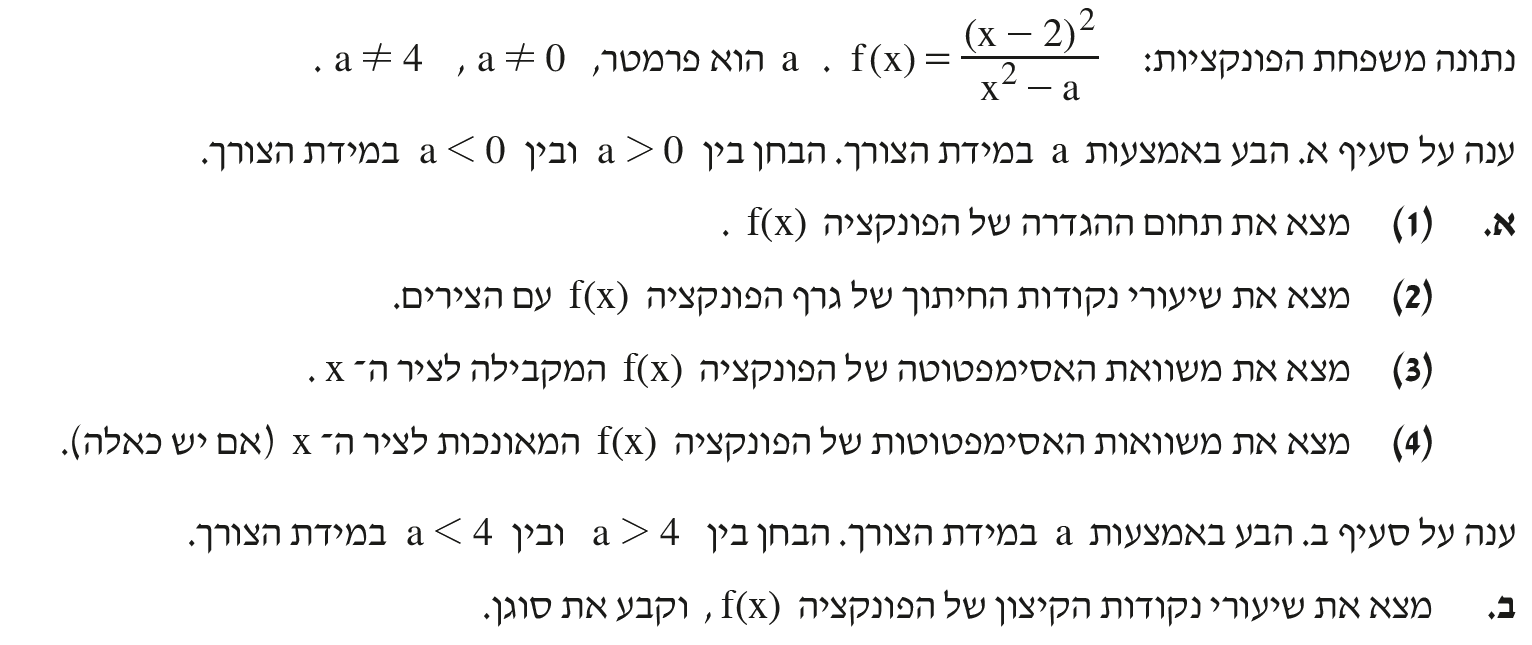
\includegraphics[width=\textwidth]{winter-2018-7a}
\end{center}

\vspace{-2ex}

\textbf{סעיף ג של השאלה מופיע בהמשך.}

\textbf{סעיף א}

$(1)$
כאשר
$a>0$,
הפונקציה לא מוגדרת עבור
$x=\pm\sqrt{a}$,
ערכים שמאפסים את המכנה.

כאשר
$a<0$,
המכנה תמיד חיובי והפונקציה מוגדרת לכל
$x$.



$(2)$
חישוב נקודת החיתוך עם ציר ה-%
$y$:
$f(0)=\disfrac{(-2)^2}{-a}=-\disfrac{4}{a}$.

חישוב נקודת החיתוך עם ציר ה-%
$x$:
כאשר 
$a<0$,
המכנה חיובית והפונקציה מתאפסת כאשר 
$x=2$.
נתון ש-%
$a\neq 4$,
ולכן גם כאשר
$a>0$,
ב-%
$x=2$
המכנה לא מתאפסת ומונה מתאפסת:
\[
f(x)=\frac{(x-2)^2}{x^2-a}=\frac{(x-2)(x-2)}{(x-\sqrt{a})(x+\sqrt{a})},\quad f(2)=0\,.
\]

$(3)$
$y=1$
היא
\asm{}
אופקית:
\[
f(x)=\frac{1-\frac{4x}{x^2}+\frac{4}{x^2}}{1-\frac{a}{x^2}}\limit{\pm\infty} = 1\,.
\]

$(4)$
כאשר 
$a<0$
הפונקציה מוגדרת לכל
$x$
ואין
\asm{}.

כאשר
$a>0$:
נתון
$a\neq 4$
כך ש-%
$\sqrt{a}\neq 2$,
לכן המונה של הפונקציה לא מתאפסת כאשר
$x\rightarrow \pm\sqrt{a}$.
יש 
\asms{}
אנכיות
$x=\pm\sqrt{a}$.

\smallskip

\textbf{סעיף ב}

\vspace{-3ex}

\erh{12pt}
\begin{equationarray*}{rcl}
f'(x)=\left(\frac{(x-2)^2}{x^2-a}\right)'&=&\frac{2(x-2)(x^2-a)-(x-2)^2\cdot 2x}{(x^2-a)^2}\\
&=&\frac{2(x-2)\,(2x-a)}{(x^2-a)^2}\,.
\end{equationarray*}

\np

נקודות הקיצון הן
$(2,0)$,
$\left(\disfrac{a}{2},\disfrac{a-4}{a}\right)$.

נחשב את הסימן של הנגזרת של המונה של הנגזרת הראשונה:
\[
(2(x-2)\,(2x-a))'=8x-2a-8\,.
\]
לפי ההנחיה בשאלה נבדוק בנפרד עבור ערכים חיוביים ושליליים של
$a$.

עבור 
$a>4$:

$8\cdot 2 - 2a - 8=2(4-a)<0$
ו-%
$(2,0)$
היא מקסימום.

$8\cdot \disfrac{a}{2} - 2a - 8=2(a-4)>0$
ו-%
$\left(\disfrac{a}{2},\disfrac{a-4}{a}\right)$
היא מינימום.

עבור 
$a<4$
הסימנים מתחלפים ו-%
$(2,0)$
היא מינימום ו-%
$\left(\disfrac{a}{2},\disfrac{a-4}{a}\right)$
היא מקסימום.

\textbf{סעיף ג}

\begin{center}
\selectlanguage{english}
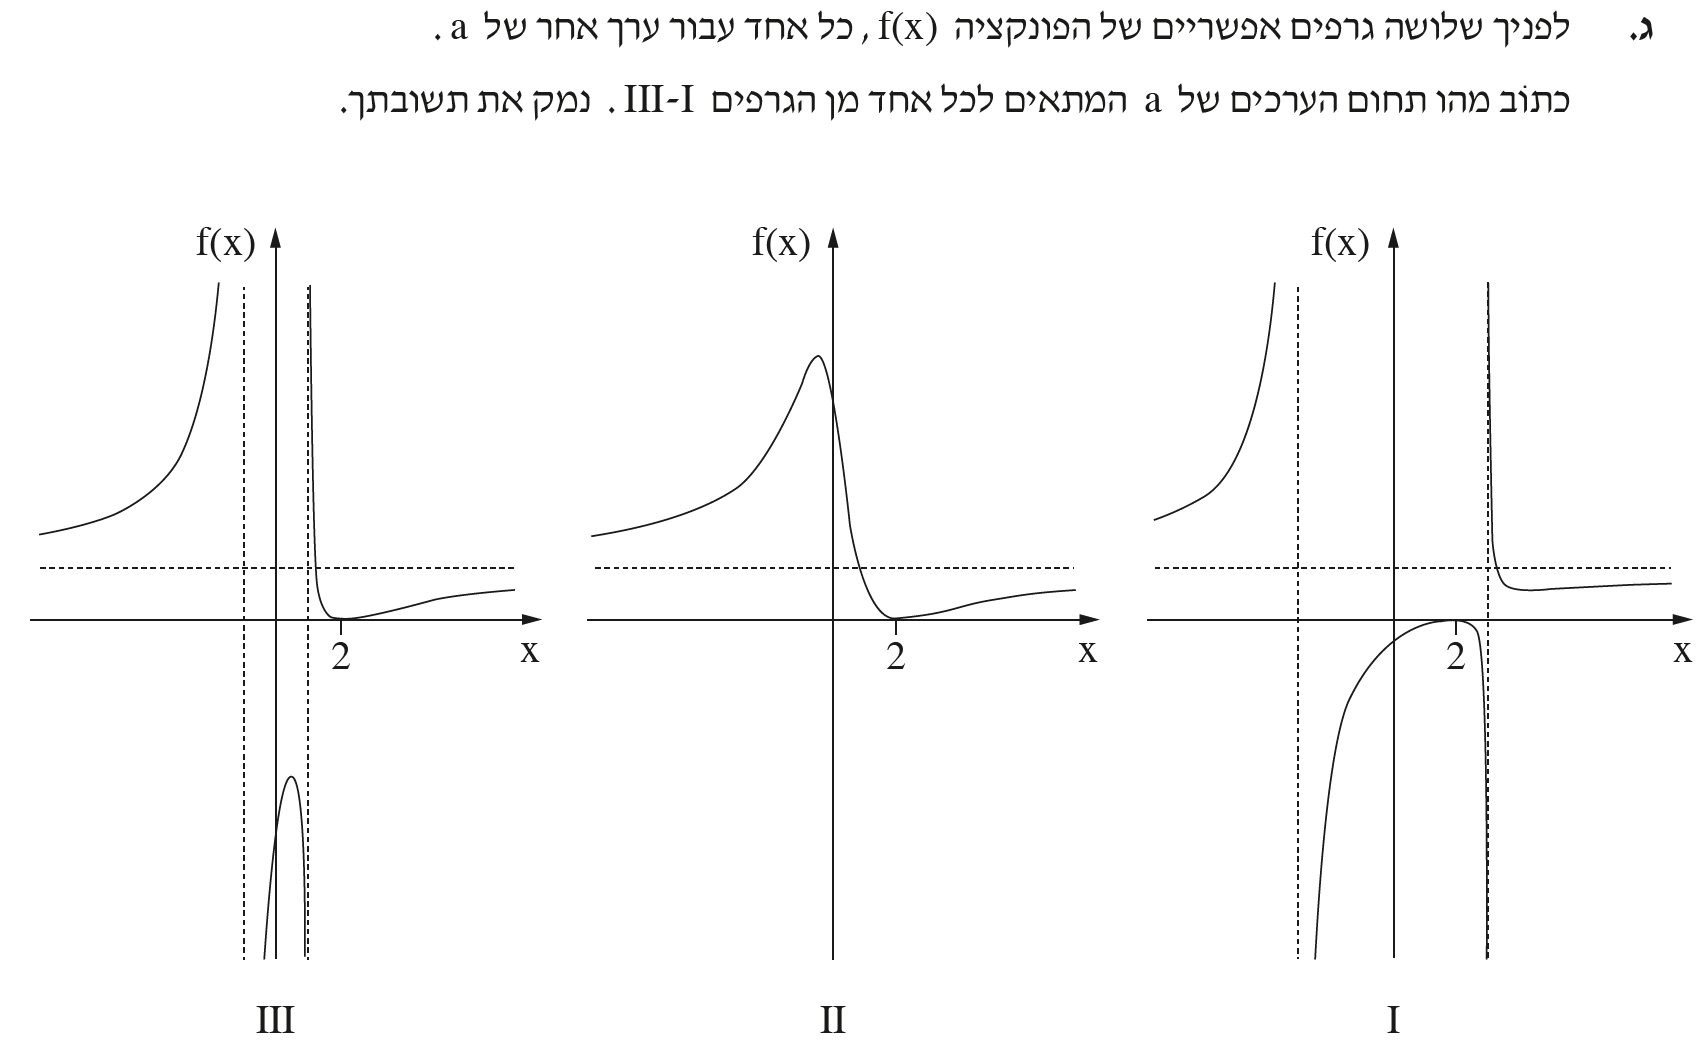
\includegraphics[width=\textwidth]{winter-2018-7b}
\end{center}


כאשר 
$a>4$
נקודות הקיצון ב-%
$(2,0)$
היא מקסימום כפי שמופיע בגרף I. כאשר 
$a<0$
הפונקציה מוגדרת כל ל-%
$x$
כפי שמופיע בגרף II. כאשר 
$0<a<4$
נקודת הקיצון ב-%
$(2,0)$
היא מינימום, ויש
\asms{}
ב-%
$x=\pm\sqrt{a}$
 כפי שמופיע בגרף III.

\np

%%%%%%%%%%%%%%%%%%%%%%%%%%%%%%%%%%%%%%%%%%%%%%%%%%%%%%%%%%%%%%%%%%%%%%

\section{קיץ תשע"ז מועד ב}

\begin{center}
\selectlanguage{english}
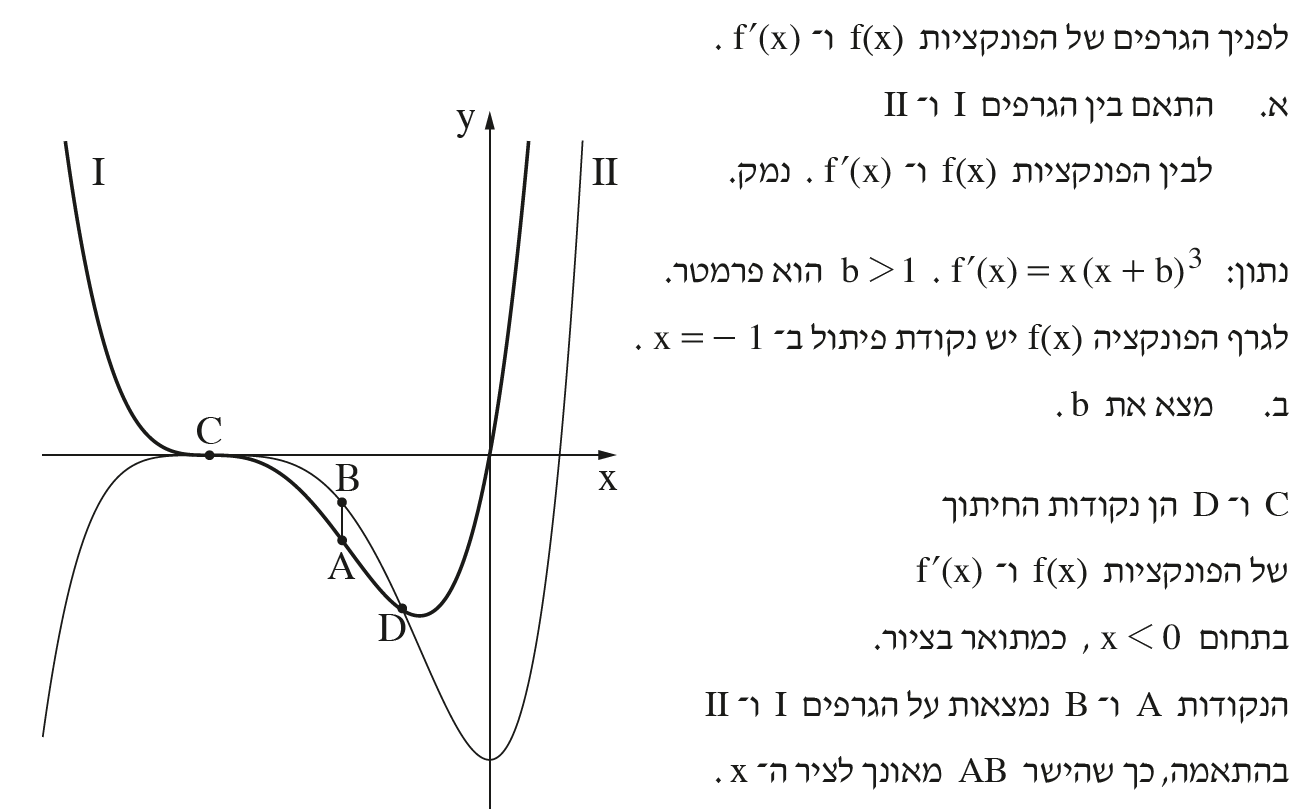
\includegraphics[width=\textwidth]{summer-2017b-7a}
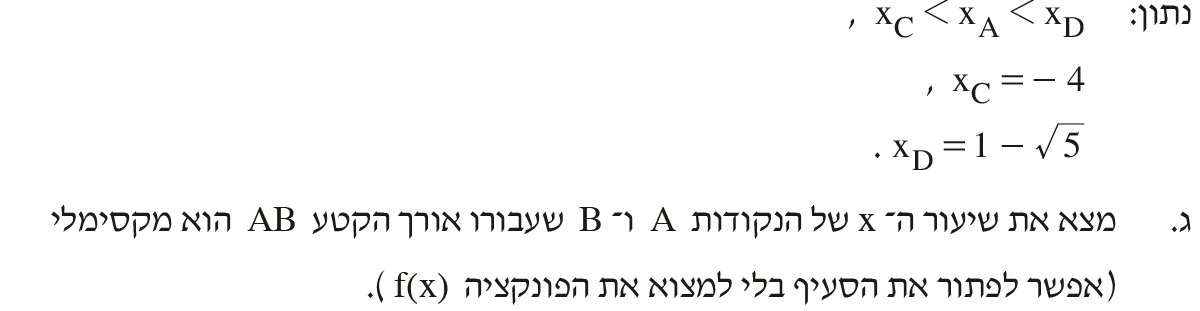
\includegraphics[width=\textwidth]{summer-2017b-7b}
\end{center}

\vspace{-2ex}

\textbf{סעיף א}

הגרף I מתאפס בנקודה 
$C$
שם לגרף II יש נקודה מקסימום. גרף I מתאפס ב-%
$(0,0)$
שם לגרף II יש נקודה מינימום. לכן, II הוא הגרף של
$f(x)$
ו-I הוא הגרף של
$f'(x)$.

\textbf{סעיף ב}

בנקודת פיתול הנגזרת השנייה מתאפסת:
\erh{2pt}
\begin{equationarray*}{rcl}
f''(x) &=& 1\cdot (x+b)^3+x\cdot 3(x+b)^2=(x+b)^2(4x+b)\\
f''(-1) &=& (b-1)^2 (b-4)=0\\
b&=&4\,,
\end{equationarray*}
כי נתון ש-%
$b>1$.

\np

\textbf{סעיף ג}

הערך המקסימלי יתקבל כאשר הנגזרת של ההפרש מאפסת. הנגזרת הראשונה, הנגזרת של
$f(x)$
נתונה, והנגזרת השנייה, הנגזרת של הנגזרת הראשונה חושבה בסעיף ב, שם קבלנו ש-%
$b=4$:
\erh{2pt}
\begin{equationarray*}{rcl}
(f(x)-f'(x))'&=& x(x+4)^3 - (x(x+4))^3)'\\
&=&x(x+4)^3 - (x+4)^2(4x+4)\\
&=&(x+4)^2(x^2-4)=0\,.
\end{equationarray*}

\vspace{-2ex}

הפתרונות הם
$x=-4,x=\pm 2$.

$x_C=-4$,
$x_D=1-\sqrt{5}=-1.24$,
ולכן הפתרון היחיד בתחום הוא 
$x=-2$.


\np

%%%%%%%%%%%%%%%%%%%%%%%%%%%%%%%%%%%%%%%%%%%%%%%%%%%%%%%%%%%%%%%%%%%%%%

\section{קיץ תשע"ז מועד א}

\begin{center}
\selectlanguage{english}
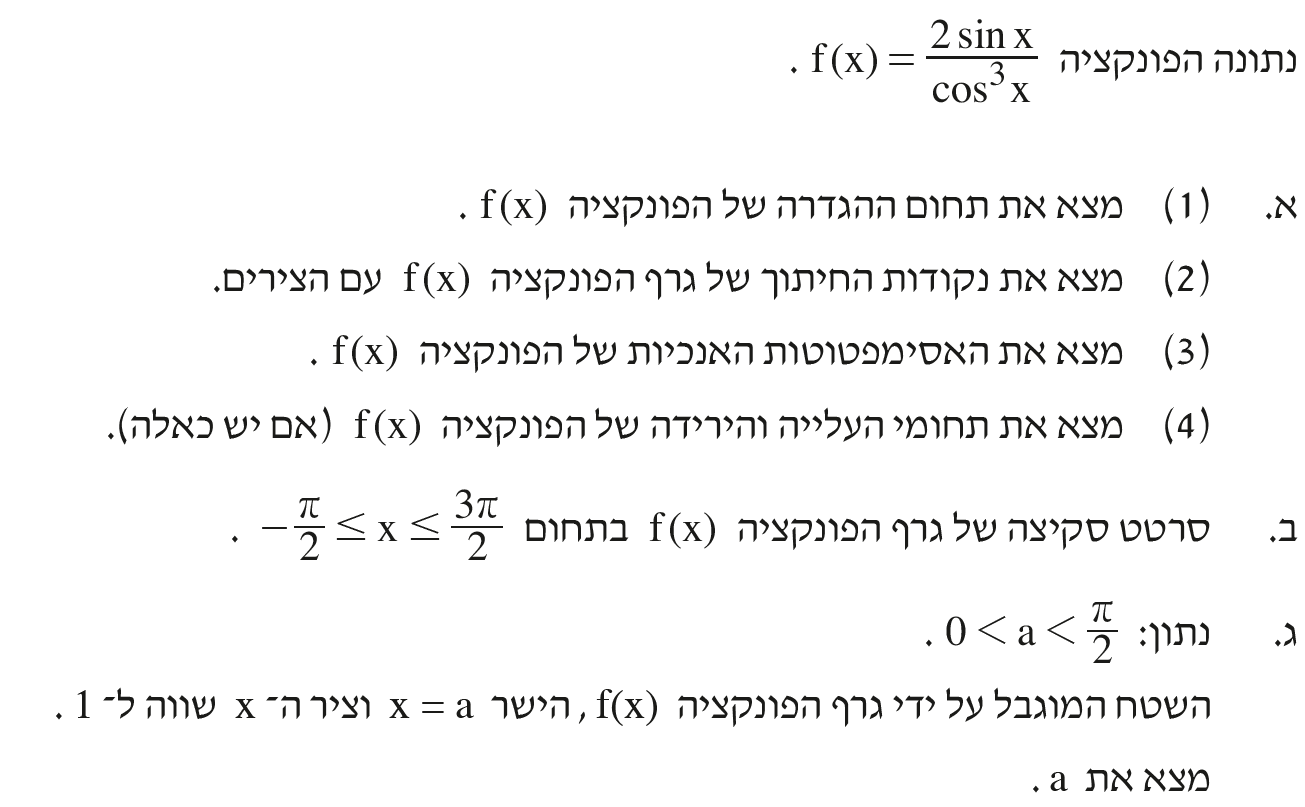
\includegraphics[width=.85\textwidth]{summer-2017a-7}
\end{center}

\vspace{-2ex}

\textbf{סעיף א}

$(1)$
הפונקציה מוגדרת כאשר המכנה לא מתאפס:
$x \neq \frac{\pi}{2} \pm n\pi$.

$(2)$
נקודות החיתוך עם ציר ה-%
$x$
הן כל הנקודות עבורן
$\sin x = 0$
ו-%
$\cos x \neq 0$,
שהן 
$x=\pm n\pi$.
כאשר 
$x=0$,
$y=0$
והנקודה היא גם נקודת חיתוך עם ציר ה-%
$y$.

$(3)$
יש
\asms{}
אנכיות ב-%
$x=\frac{\pi}{2} \pm n\pi$
כי הפונקציה שאופת לאינסוף שם.

אין 
\asm{}
אופקיות: כאשר
$x\rightarrow \pm \infty$,
הפונקציה לא חסומה ושואפת לאינסוף שוב ושוב.

$(4)$
\[
f'(x)=\frac{(2\cos x\cdot\cos^3 x) - (2\sin x \cdot 3\cos^2 x \cdot -\sin x)}{\cos^6 x}=\frac{2\cos^4 x + 6\sin^2 x\cos^2 x}{\cos^6 x}\,.
\]
כל הגורמים בביטוי חיוביים כי הם חזקות זוגיות של פונקציות טריגונומטריות, ולכן הפונקציה עולה בכל תחום ההגדרה.

\np

\textbf{סעיף ב}

הסרטוט מבוסס על נקודות החיתוך עם ציר ה-%
$x$,
ה%
\asms{}
האנכיות, והעובדה שהפונקציה תמיד עולה.

\begin{center}
\selectlanguage{english}
\begin{tikzpicture}%[scale=.8]
\begin{axis}[
    trig format plots=rad,
    axis lines=center,
    xmin = -2,
    xmax = 5,
    xtick={-1.57,0,1.57,3.14,4.71},
    xticklabels={$-\frac{\pi}{2}$,$0$, $\frac{\pi}{2}$,$\pi$,$\frac{3\pi}{2}$},
    ymin = -10.1,
    ymax = 10.1,
    ymajorticks=false,
    xticklabel style={anchor=north west,},
]
\addplot [
    domain=-1.4:1.4,
    samples=50, 
]
{(2*sin(x))/(cos(x)^3)};
\addplot [
    domain=1.7:4.55,
    samples=50, 
]
{(2*sin(x))/(cos(x)^3)};
\draw[dashed,thick] (axis cs:-1.57,-10) -- (axis cs:-1.57,10);
\draw[dashed,thick] (axis cs:1.57,-10) -- (axis cs:1.57,10);
\draw[dashed,thick] (axis cs:4.71,-10) -- (axis cs:4.71,10);
\fill (axis cs:0,0) circle(1.5pt);
\fill (axis cs:3.14,0) circle(1.5pt);
\end{axis}
\end{tikzpicture}
\end{center}


\textbf{סעיף ג}
\[
\int_0^a \frac{2\sin x}{\cos^3 x}dx = \left. \cos^{-2} x \right|_0^a=\frac{1}{\cos^2 a}-\frac{1}{1^2}=1\,.
\]

מכאן ש-%
$\cos a=\sqrt{\disfrac{1}{2}}=\disfrac{\sqrt{2}}{2}$,
והפתרון היחיד בתחום
$0<a<\disfrac{\pi}{2}$
הוא
$a=\disfrac{\pi}{4}$.

\np


%%%%%%%%%%%%%%%%%%%%%%%%%%%%%%%%%%%%%%%%%%%%%%%%%%%%%%%%%%%%%%%%%%%%%%

\section{חורף תשע"ז}

\begin{center}
\selectlanguage{english}
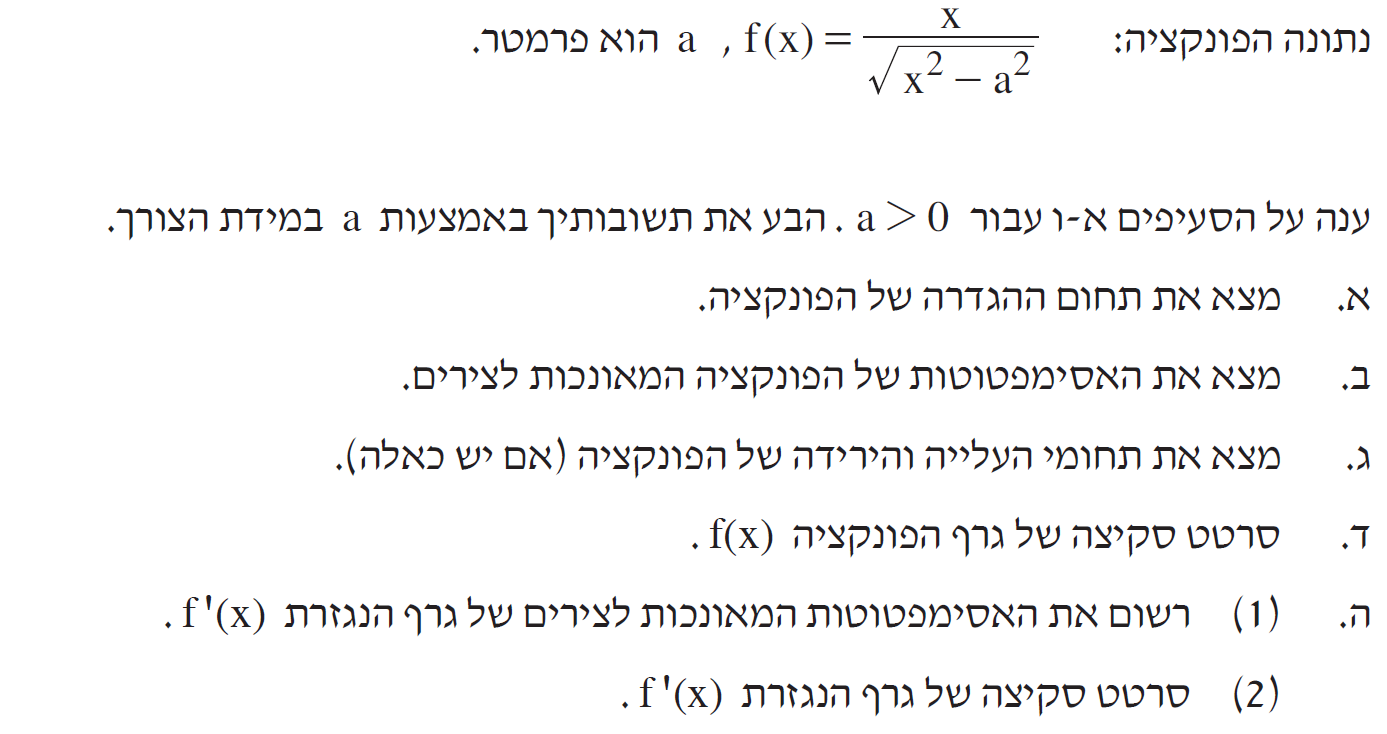
\includegraphics[width=.85\textwidth]{winter-2017-7a}
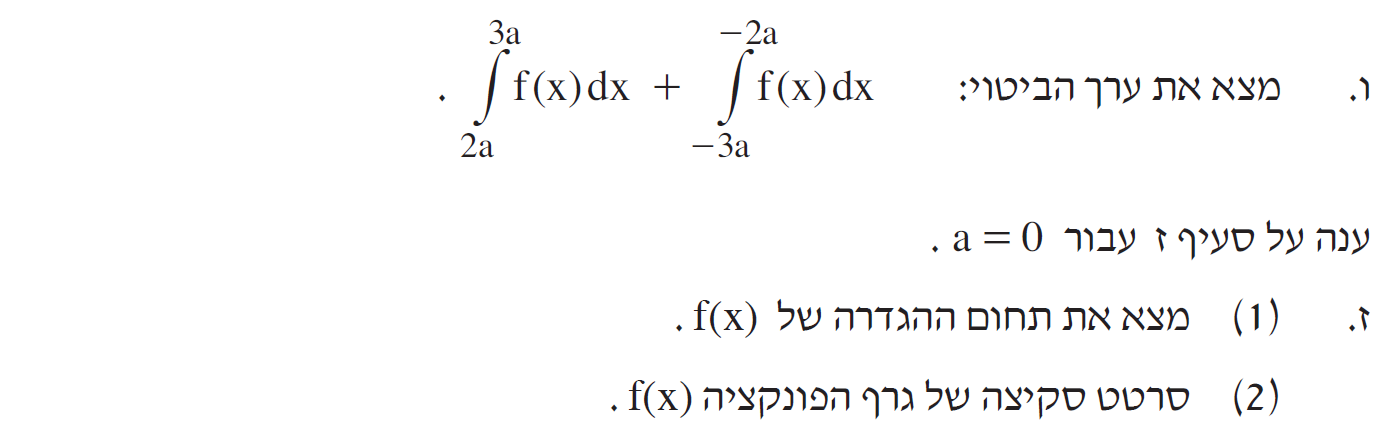
\includegraphics[width=.85\textwidth]{winter-2017-7b}
\end{center}

\vspace{-2ex}

\textbf{סעיף א}

הפונקציה לא מוגדרת כאשר המכנה מתאפס
$x=\pm a$
או כאשר הביטוי בשורש שלילי
$|x|\leq a$.
תחום ההגדרה הוא
$|x|>a$.

\textbf{סעיף ב}

המכנה תמיד חיובי אבל ה-%
$x$
במונה גורם לסימן של ה%
\asms{}
האכניות להיות תלויות בכיוון ההתקרבות לנקודות בהן הפונקציה לא מוגדרת:
\[
\frac{\disfrac{x}{\sqrt{x^2}}}{\sqrt{1-\disfrac{a^2}{x^2}}}=\disfrac{\disfrac{x}{|x|}}{\sqrt{1-\disfrac{a^2}{x^2}}}\limit{\pm a}\pm 1\,.
\]
ה%
\asm{}
האופקית היא
$y=\pm 1$,
כאשר הסימן הוא לפי כיוון השאיפה לאינסוף:
\[
\frac{x}{\sqrt{x^2-a}}\approx \frac{x}{\sqrt{x^2}}\limit{\pm\infty} \pm 1\,.
\]
\textbf{סעיף ג}

נבדוק את הסימן של הנגזרת הראשונה:
\[
f'(x)=1\cdot(x^2-a^2)^{-\frac{1}{2}} + x\cdot \left(-\frac{1}{2}\right)(x^2-a^2)^{-\frac{3}{2}}\cdot 2x=\frac{-a^2}{(x^2-a^2)^{\frac{3}{2}}}\,.
\]
המכנה חיובי והמונה שלילי, לכן הנגזרת שלילי והפונקציה יורדת בכל תחום ההגדרה שלה.

\np

\textbf{סעיף ד}

יש לנו את ה%
\asms{}
מסעיף ב, ומסעיף ג אנו יודעים שהפונקציה תמיד יורדת:

\vspace{-1ex}

\begin{center}
\selectlanguage{english}
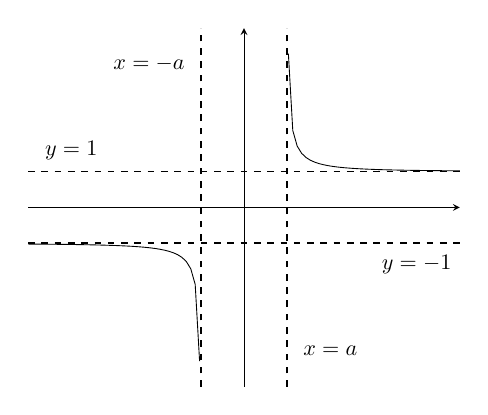
\begin{tikzpicture}[scale=.8]
\begin{axis}[
    axis lines=center,
    xmin = -5,
    xmax = 5,
    ymin = -5,
    ymax = 5,
    xmajorticks=false,
    ymajorticks=false,
]
\addplot [
    domain=-5:-.01,
    samples=50, 
]
{(x)/(sqrt(x^2-1))};
\addplot [
    domain=.01:5,,
    samples=50, 
]
{(x)/(sqrt(x^2-1))};
\draw[dashed,thick] (axis cs:-5,1) -- (axis cs:5,1);
\draw[dashed,thick] (axis cs:-5,-1) -- (axis cs:5,-1);
\node at (axis cs:-4,1.6) {$y=1$};
\node at (axis cs:4,-1.6) {$y=-1$};
\draw[dashed,thick] (axis cs:1,-5) -- (axis cs:1,5);
\draw[dashed,thick] (axis cs:-1,-5) -- (axis cs:-1,5);
\node at (axis cs:-2.2,4) {$x=-a$};
\node at (axis cs:2,-4) {$x=a$};
\end{axis}
\end{tikzpicture}
\end{center}

\vspace{-2ex}

\textbf{סעיף ה}

$(1)$
המכנה של 
$f'(x)$
מתאפסת כאשר 
$x=\pm a$
ולכן יש 
\asms{}
אנכיות ב-%
$x=\pm a$.

כאשר
$x\rightarrow \pm \infty$,
המונה חיובי והמכנה שואפת ל-%
$+\infty$,
ולכן יש
\asm{}
אופקית ב-%
$y=0$.

$(2)$
לפי סעיף ג הנגזרת תמיד שלילי ויש 
\asms{}
ב-%
$\pm a$:

\vspace{-1ex}

\begin{center}
\selectlanguage{english}
\begin{tikzpicture}[scale=.8]
\begin{axis}[
    axis lines=center,
    xmin = -5,
    xmax = 5,
    ymin = -5,
    ymax = 5,
    xmajorticks=false,
    ymajorticks=false,
]
\addplot [
    domain=-5:-.01,
    samples=50, 
]
{(-1)/(sqrt(x^2-1))};
\addplot [
    domain=.01:5,,
    samples=50, 
]
{(-1)/(sqrt(x^2-1))};
\draw[dashed,thick] (axis cs:1,-5) -- (axis cs:1,5);
\draw[dashed,thick] (axis cs:-1,-5) -- (axis cs:-1,5);
\node at (axis cs:-2.2,4) {$x=-a$};
\node at (axis cs:2,-4) {$x=a$};
\end{axis}
\end{tikzpicture}
\end{center}

\vspace{-2ex}

\textbf{סעיף ו}

\[
f(-x) = \frac{-x}{(-x)^2-a^2}= -\frac{x}{x^2-a^2} = -f(x)\,.
\]
הפונקציה אי-זוגיות ולכן אינטגרציה של קטעים סימטריים מצדי ציר ה-%
$y$
מצטצמים והסכום
$0=$.

\textbf{סעיף ז}

$(1)$
$f(x)=\disfrac{x}{\sqrt{x^2}}=\disfrac{x}{|x|}=\pm 1$
עבור 
$x\neq 0$.
כאשר הסימן הוא הסימן של
$x$.

$(2)$
\begin{center}
\selectlanguage{english}
\begin{tikzpicture}[scale=.8]
\begin{axis}[
    axis lines=center,
    xmin = -5,
    xmax = 5,
    ymin = -2,
    ymax = 2,
    xmajorticks=false,
    ymajorticks=false,
]
\draw[thick] (axis cs:-5,-1) -- (axis cs:-.12,-1);
\draw[thick] (axis cs:.12,1) -- (axis cs:5,1);
\draw (axis cs:0,1) circle(3pt);
\draw (axis cs:0,-1) circle(3pt);
\end{axis}
\end{tikzpicture}
\end{center}

\np



%%%%%%%%%%%%%%%%%%%%%%%%%%%%%%%%%%%%%%%%%%%%%%%%%%%%%%%%%%%%%%%%%%%%%%

\section{קיץ תשע"ו מועד ב}

\begin{center}
\selectlanguage{english}
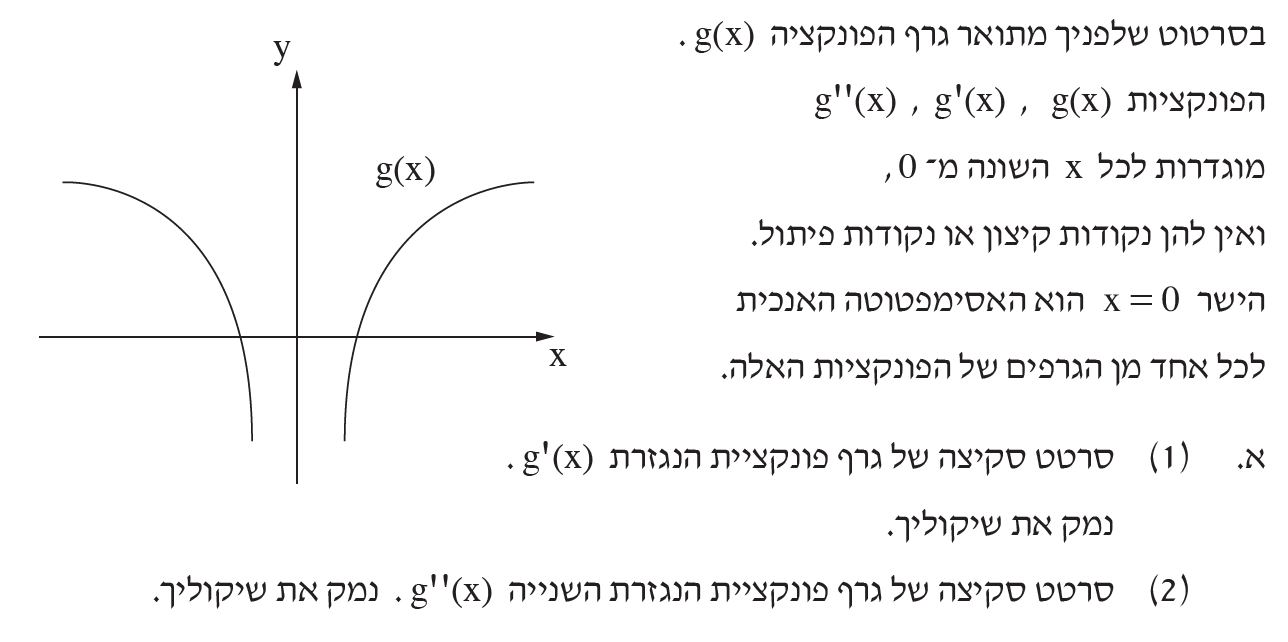
\includegraphics[width=.95\textwidth]{summer-2016b-7a}
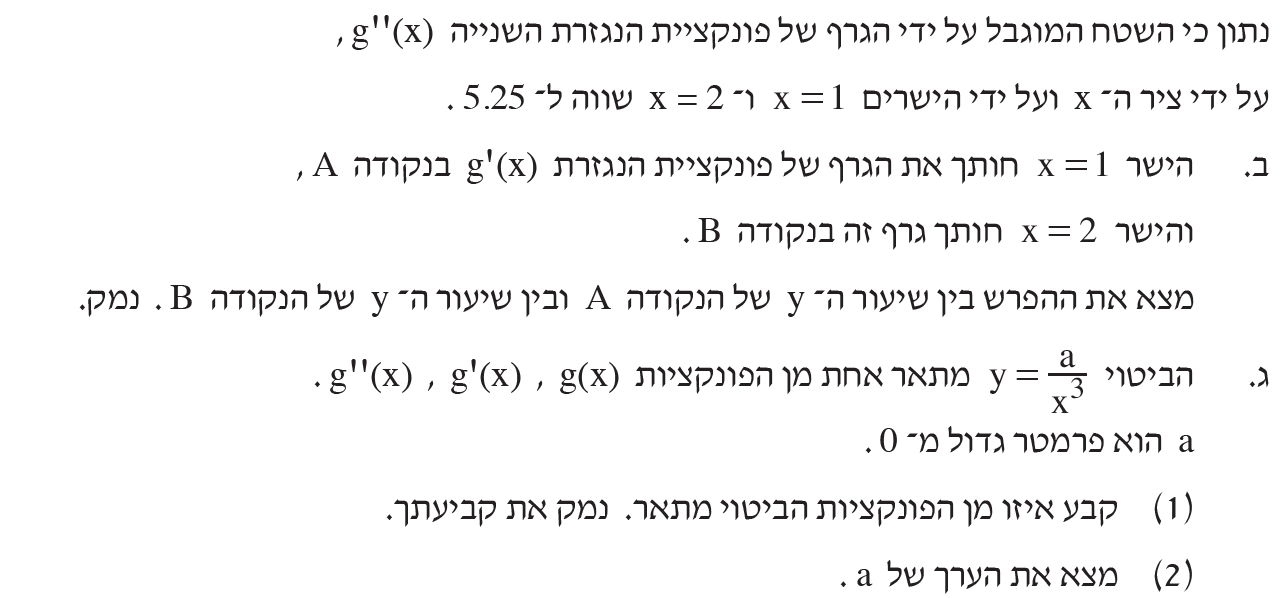
\includegraphics[width=.95\textwidth]{summer-2016b-7b}
\end{center}

\vspace{-1ex}

נוח לי להציג את כל שלושת הגרפים במערכת צירים אחת, למרות שאיפיון הגרפים יתברר רק במהלך פתרון השאלה. 
$g(x)$:
קו רגיל.
$g'(x)$:
קו מקווקוו.
$g''(x)$:
קו מנוקד.

\begin{center}
\selectlanguage{english}
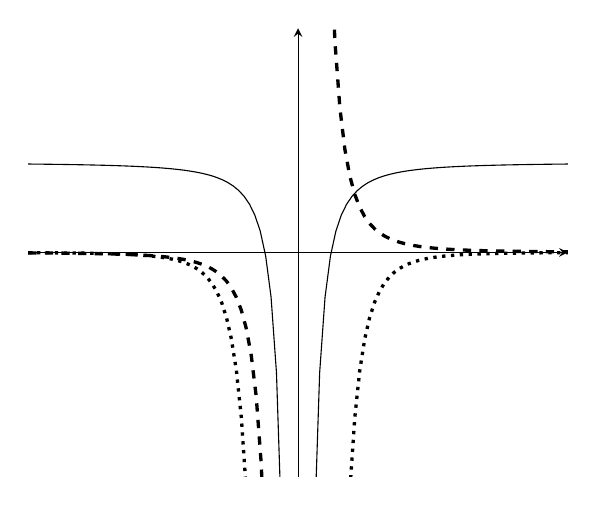
\begin{tikzpicture}%[scale=1.1]
\begin{axis}[
    axis lines=center,
    xmin = -5,
    xmax = 5,
    ymin = -20,
    ymax = 20,
    xmajorticks=false,
    ymajorticks=false,
]
\addplot [
    domain=-5:-.1,
    samples=50, 
]
{(-3)/(x^2)+8};
\addplot [
    domain=.1:5,
    samples=50, 
]
{(-3)/(x^2)+8};
\addplot [
    domain=-5:-.5,
    samples=50, 
    very thick,
    dashed,
]
{(6)/(x^3)};
\addplot [
    domain=.5:5,
    samples=50, 
    very thick,
    dashed,
]
{(6)/(x^3)};
\addplot [
    domain=-5:-.5,
    samples=50,
    very thick,
    dotted,
]
{(-18)/(x^4)};
\addplot [
    domain=.5:5,
    samples=50, 
    very thick,
    dotted,
]
{(-18)/(x^4)};
\end{axis}
\end{tikzpicture}
\end{center}

\np

\textbf{סעיף א}

$(1)$
משמאל לימין עבור ערכים שליליים של 
$x$,
השיפוע של פונקציה שלילי ויורדת תמיד ולכן הנגזרת תמיד שלילית. ערכה של הנגזרת מתחילה קרוב לאפס, יורדת לאט ואז יורדת מהר ושואפת 
$-\infty$.

משמאל לימין עבור ערכים חיוביים של 
$x$,
השיפוע של פונקציה חיובי ויורדת תמיד ולכן הנגזרת חיובית. ערכה של הנגזרת מתחילה קרוב ל-%
$+\infty$,
יורדת מהר ואז יורדת לאט ושואפת 
$0$.


$(2)$
משמאל לימין עבור ערכים שליליים של 
$x$,
הנגזרת הראשונה מתנהגות בדיוק כמו הפונקציה, ולכן הגרף של הנגזרת השנייה דומה לגרף של הנגזרת הראשונה.

משמאל לימין עבור ערכים חיוביים של 
$x$,
השיפוע של הנגזרת הראשונה שלילי ועולה תמיד ולכן הנגזרת השנייה שלילית. ערכה של הנגזרת השנייה מתחילה קרוב ל-%
$-\infty$,
עולה מהר ואז עולה לאט ושואפת 
$0$.

\medskip

\textbf{סעיף ב}

התרשים להלן מראה את
$g'(x),g''(x)$
עבור ערכים חיוביים. השטח המתואר מודגש.

\begin{center}
\selectlanguage{english}
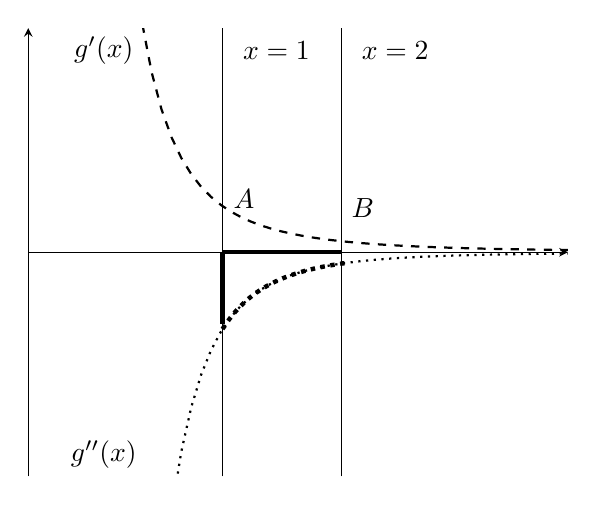
\begin{tikzpicture}%[scale=1.1]
\begin{axis}[
    axis lines=center,
    xmin = 0,
    xmax = 5,
    ymin = -5,
    ymax = 5,
    xmajorticks=false,
    ymajorticks=false,
]
\addplot [
    domain=.5:5,
    samples=50, 
    thick,
    dashed,
]
{(6)/(x^3)};
\addplot [
    domain=.5:5,
    samples=50, 
    thick,
    dotted,
]
{(-18)/(x^4)};
\draw (axis cs:1.8,-5) -- (axis cs:1.8,5);
\draw (axis cs:2.9,-5) -- (axis cs:2.9,5);
\node at (axis cs:2.3,4.5) {$x=1$};
\node at (axis cs:3.4,4.5) {$x=2$};
\node at (axis cs:.7,4.5) {$g'(x)$};
\node at (axis cs:.7,-4.5) {$g''(x)$};
\addplot [
    domain=1.8:2.95,
    samples=50, 
    ultra thick,
    dotted,
]
{(-18)/(x^4)};
\draw[ultra thick] (axis cs:1.8,0) -- (axis cs:1.8,-1.61);
\draw[ultra thick] (axis cs:1.8,0) -- (axis cs:2.9,0);
\node at (axis cs:2,1.2) {$A$};
\node at (axis cs:3.1,1) {$B$};
\end{axis}
\end{tikzpicture}
\end{center}
חישוב השטח:
\[
S=\int_1^2 -g''(x) dx = \left.-g'(x)\rule{0pt}{12pt}\right|_1^2=g'(1)-g'(2)=5.25\,.
\]
אבל זה בדיוק ההפרש בין ערך ה-%
$y$
של הנקודה
$A$
לבין ערך ה-%
$y$
של נקודה 
$B$.

\medskip

\textbf{סעיף ג}

$(1)$
הביטוי לא מתאפס ולכן לא יוכל להיות
$g(x)$.
הביטוי חיובי עבור
$x>0$
ולכן לא יכול להיות
$g''(x)$.
נשאר 
$g'(x)=\disfrac{a}{x^3}$.

$(2)$
מסעיף ב:
\erh{12pt}
\begin{equationarray*}{rcl}
g'(1)-g'(2)&=&5.25\\
\frac{a}{1^3}-\frac{a}{2^3}&=&\frac{21}{4}\\
a&=&\frac{8}{7}\cdot \frac{21}{4}=6\,.
\end{equationarray*}

\np

%%%%%%%%%%%%%%%%%%%%%%%%%%%%%%%%%%%%%%%%%%%%%%%%%%%%%%%%%%%%%%%%%%%%%%

\section{קיץ תשע"ו מועד א}

\begin{center}
\selectlanguage{english}
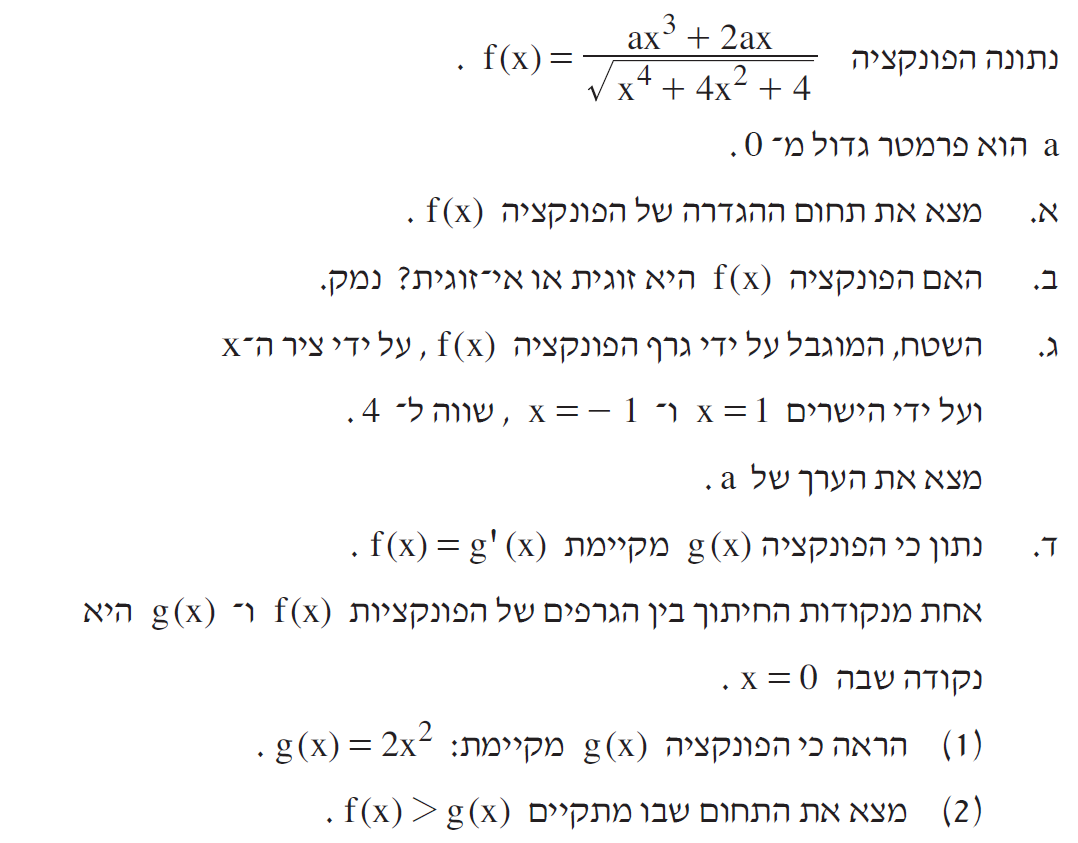
\includegraphics[width=.85\textwidth]{summer-2016a-7}
\end{center}

\vspace{-2ex}

\textbf{סעיף א}

השאלה פשוטה יותר אם נשים לב ש:
\[
f(x)=\frac{ax^3+2ax}{\sqrt{x^4+4x^+4}}=\frac{ax (x^2+2)}{\sqrt{(x^2+2)^2}}=\frac{ax (x^2+2)}{x^2+2}=ax\,.
\]
אנחנו מסתמכים על העובדה ש-%
$x^2+2>0$
כך שניתן לחשב את השורש במכנה ולצמצם את השבר, בלי לשנות את התכונות של הפונקציה.

ברור ש-%
$f(x)$
מוגדרת לכל
$x$.

\medskip

\textbf{סעיף ב}

$x^2+2$
זוגית כך שהזוגיות תלוייה רק בזוגיות של
$ax$.
$a(-x)=-(ax)$
והפונקציה אי-זוגיות.
\medskip

\textbf{סעיף ג}

כאן צריך להיזהר.
\textbf{האינטגרל}
של פונצקיה אי-זוגית בתחום הסימטרי בין
$-k$
ל-%
$k$
הוא אפס כי התרומה של הערכים החיוביים והשליליים מצטמצמים. אבל
\textbf{השטח}
התחום על ידי תחום סימטרי כולל את השטח מתחת לציר ה-%
$x$
והשטח מעל לציר ה-%
$x$.
עבור פונקציה אי-זוגית, השטחים שווים.
\[
S = 2\int_0^1 ax \,dx = \left.ax^2\rule{0pt}{12pt}\right|_0^1=a=4\,.
\]

\np

\begin{center}
\selectlanguage{english}
\begin{tikzpicture}%[scale=1.1]
\begin{axis}[
    axis lines=center,
    xmin = -2,
    xmax = 2,
    ymin = -5,
    ymax = 5,
    xmajorticks=false,
    ymajorticks=false,
]
\addplot [
    domain=-3:3,
    samples=50, 
]
{4*x};
\draw[thick,dashed] (axis cs:-1,-5) -- (axis cs:-1,0);
\draw[thick,dashed] (axis cs:1,0) -- (axis cs:1,5);
\end{axis}
\end{tikzpicture}
\end{center}

\textbf{סעיף ד}

$(1)$
\[
g(x)=\int g'(x) \, dx = \int f(x)\, dx = \int ax\, dx = \frac{1}{2}ax^2 + c\,.
\]
לפי הנתון על נקודת החיתוך:
\[
f(0)=a\cdot 0 = \frac{1}{2}\cdot a\cdot 0^2 + c= g(0)\,,
\]
ו-%
$c=0$.
לכן
$g(x)=\frac{1}{2}\cdot 4x^2+0 = 2x^2$.


$(2)$
\erh{2pt}
\begin{equationarray*}{rcl}
f(x)&\stackrel{?}{>}&g(x)\\
4x&\stackrel{?}{>}&2x^2\\
2&>&x\,.
\end{equationarray*}
אפשר לצמצם
$x$
כי 
$f(0)= g(0) = 0$,
ולכן
$x=0$
אינו ערך עבורו
$f(x)>g(x)$.

עבור
$x<0$,
$f(x)$
שלילי ו-%
$g(x)$
חיובי, וברור ש-%
$f(x)\not > g(x)$.
לכן התחום בו
$f(x)>g(x)$
הוא
$0<x<2$.

\np

%%%%%%%%%%%%%%%%%%%%%%%%%%%%%%%%%%%%%%%%%%%%%%%%%%%%%%%%%%%%%%%%%%%%%%

\section{חורף תשע"ו}

\begin{center}
\selectlanguage{english}
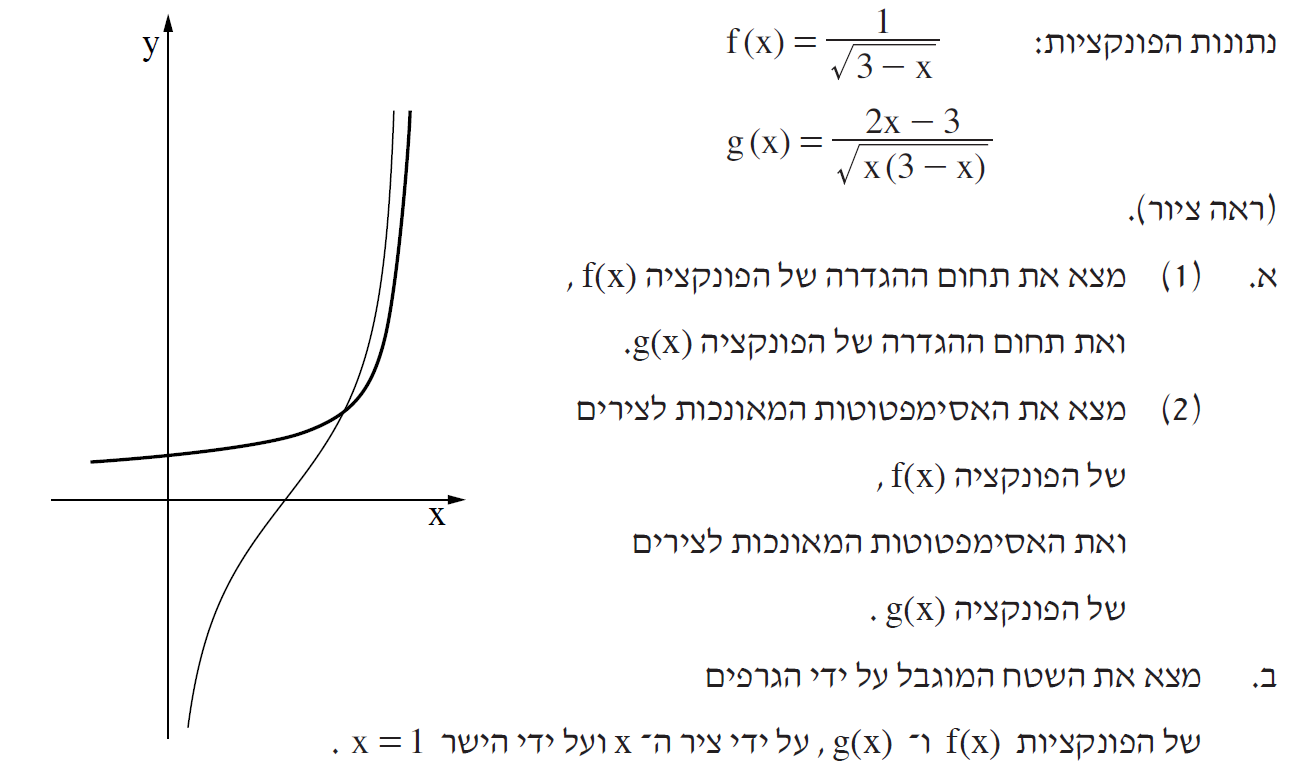
\includegraphics[width=\textwidth]{winter-2016-7a}
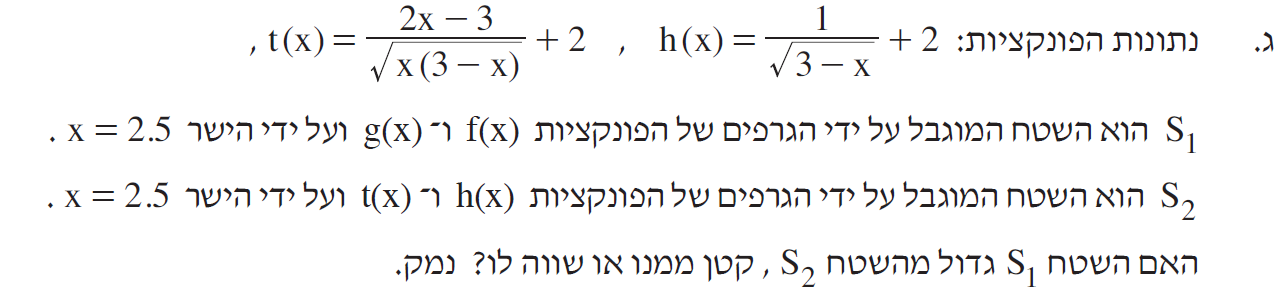
\includegraphics[width=\textwidth]{winter-2016-7b}
\end{center}

\vspace{-2ex}

\textbf{סעיף א}

$(1)$
$f(x)$:
השורש לא שלילי לכן
$x\leq 3$.
המכנה לא אפס לכן
$x\neq 3$.
ביחד
$x<3$.

$g(x)$:
כמו עבור 
$f(x)$,
$x<3$.
אבל
$x$
בשורש לא יכול להיות אפס. כמו כן, עבור
$x<0$,
בגלל ש-%
$3-x>0$
אנו מקבלים
$x(3-x)<0$,
והשורש לא מוגדר. תחום ההגדרה הוא
$0<x<3$.

$(2)$
\asms{}
אנכיות: 
$x=3$
מאפס את המכנה של שתי הפונקציות, ו-%
$x=0$
מאפס גם את 
$g(x)$.
בכל אחד מהערכים האלה המונה לא מתאפס ולכן הם מגדירים 
\asms{}.

\asms{}
אופקיות: שתי הפונקציות לא מוגדרות עבור
$x>3$
ולכן אין
\asms{}
כאשר
$x\rightarrow +\infty$.
כאשר
$x\rightarrow -\infty$,
$f(x)\rightarrow 0$,
ולכן יש ל-%
$f(x)$
\asm{}
אופקית 
$y=0$.
הפונקציה 
$g(x)$
איננה מוגדרת עבור
$x<0$
ולכן אין 
\asm{}
כאשר 
$x\rightarrow -\infty$.



\textbf{סעיף ב}

השטח התחום גם על ידי ציר ה-%
$x$
בתרשים גבולות השטח מסומנים בקו עבה, וברור שצריך להחשב בשני חלקים. אחד מ-%
$x=1$
ועד לנקודת החיתוך של
$g(x)$
עם ציר ה-%
$x$,
והשני, ההמשך עד לנקודת החיתוך של שתי הפונצקיות.

\begin{center}
\selectlanguage{english}
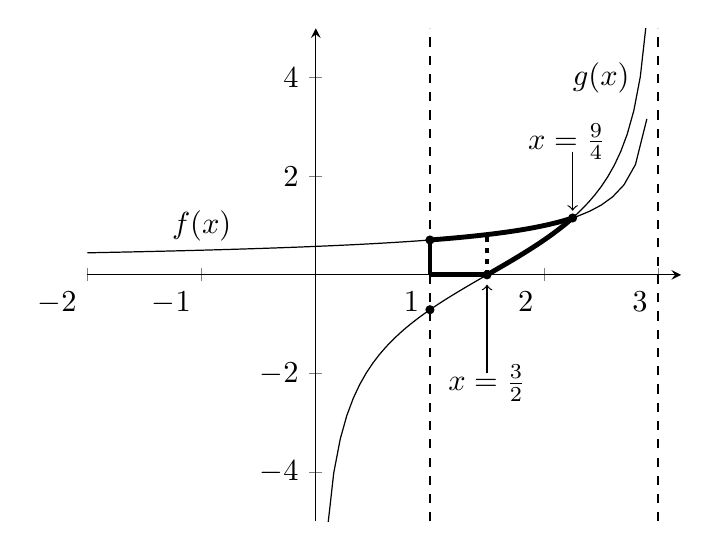
\begin{tikzpicture}[scale=1.1]
\begin{axis}[
    axis lines=center,
    xmin = -2,
    xmax = 3.2,
    ymin = -5,
    ymax = 5,
    xticklabel style={anchor=north east},
]
\addplot [
    domain=-2:2.9,
    samples=50, 
]
{(1)/sqrt(3-x)};
\addplot [
    domain=.1:2.9,
    samples=50, 
]
{(2*x-3)/sqrt(x*(3-x))};
\draw[dashed,thick] (axis cs:3,-5) -- (axis cs:3,5);
\draw[dashed,thick] (axis cs:1,-5) -- (axis cs:1,5);
\draw[dotted,ultra thick] (axis cs:1.5,0) -- (axis cs:1.5,.816);
\fill (axis cs:1,.707) circle(1.5pt);
\fill (axis cs:1,-.707) circle(1.5pt);
\fill (axis cs:1.5,0) circle(1.5pt);
\fill (axis cs:2.25,1.154) circle(1.5pt);
\node at (axis cs:-1,1) {$f(x)$};
\node at (axis cs:2.5,4) {$g(x)$};
\draw[->] (axis cs:1.5,-2) -- (axis cs:1.5,-.2);
\node at (axis cs:1.5,-2.2) {$x=\frac{3}{2}$};
\draw[->] (axis cs:2.25,2.5) -- (axis cs:2.25,1.3);
\node at (axis cs:2.2,2.7) {$x=\frac{9}{4}$};
\addplot [
    domain=1:2.25,
    samples=30, 
    ultra thick,
]
{(1)/sqrt(3-x)};
\addplot [
    domain=1.5:2.25,
    samples=30, 
    ultra thick,
]
{(2*x-3)/sqrt(x*(3-x))};
\draw[ultra thick] (axis cs:1,0) -- (axis cs:1.5,0);
\draw[ultra thick] (axis cs:1,0) -- (axis cs:1,.707);
\end{axis}
\end{tikzpicture}
\end{center}
נקודת החיתוך של
$g(x)$
עם ציר ה-%
$x$:
המכנה חיובי בתחום ההגדרה והמונה מתאפס כאשר
$x=\frac{3}{2}$.

נחשב את נקודת החיתוך של שתי הפונקציות:
\[
\frac{1}{\sqrt{3-x}}=\frac{2x-3}{\sqrt{x(3-x)}}\,.
\]
בתחום ההגדרה,
$x$
ו-%
$3-x$
חיוביים. נצמצם
$\sqrt{3-x}$,
נעלה בחזקת 
$2$
כדי להיפטר מהשורש, ונקבל משוואה ריבועית:
\[
4x^2-13x+9=(4x-9)(x-1)=0\,
\]
שיש לה שני פתרונות
$x=1, x=\frac{9}{4}$.
בדיקה מראה ש-%
$f(1)=1, g(1) = -1$,
כך שאין חיתוך בנקודה זו. נקודת החיתוך היא
$(\disfrac{9}{4},\disfrac{2}{\sqrt{3}})$.

נחשב את שני חלקי השטח בנפרד:
\erh{14pt}
\begin{equationarray*}{l}
S_1=\int_1^{\frac{3}{2}} \left(\frac{1}{\sqrt{3-x}}-0\right) \, dx =\left. -2\sqrt{3-x}\right|_1^{\frac{3}{2}}=-2\left(\sqrt{\frac{3}{2}} - \sqrt{2}\right)=0.379\\
S_2=\int_\frac{3}{2}^\frac{9}{4} \left(\frac{1}{\sqrt{3-x}}-\frac{2x-3}{\sqrt{x(3-x)}}\right)\, dx  =-2\left.\left(\sqrt{3-x}-\sqrt{x(3-x)} \right)\right|_{\frac{3}{2}}^{\frac{9}{4}}=\\
\quad\quad(-1.732+2.598)+(2.449-3)=0.315\\
S=0.379+0.315=0.694\,.
\end{equationarray*}
\textbf{סעיף ג}

בניגוד לשאלה בסעיף ב, כאן הצירים לא תוחמים את השטח. השטח מחושב על ידי ההפרש בערכי הפונקציות, ולכן הוספות קבוע לפונקציות מצטמצם וערך השטח לא משתנה.


\np

%%%%%%%%%%%%%%%%%%%%%%%%%%%%%%%%%%%%%%%%%%%%%%%%%%%%%%%%%%%%%%%%%%%%%%

\section{קיץ תשע"ה מועד ב}

\begin{center}
\selectlanguage{english}
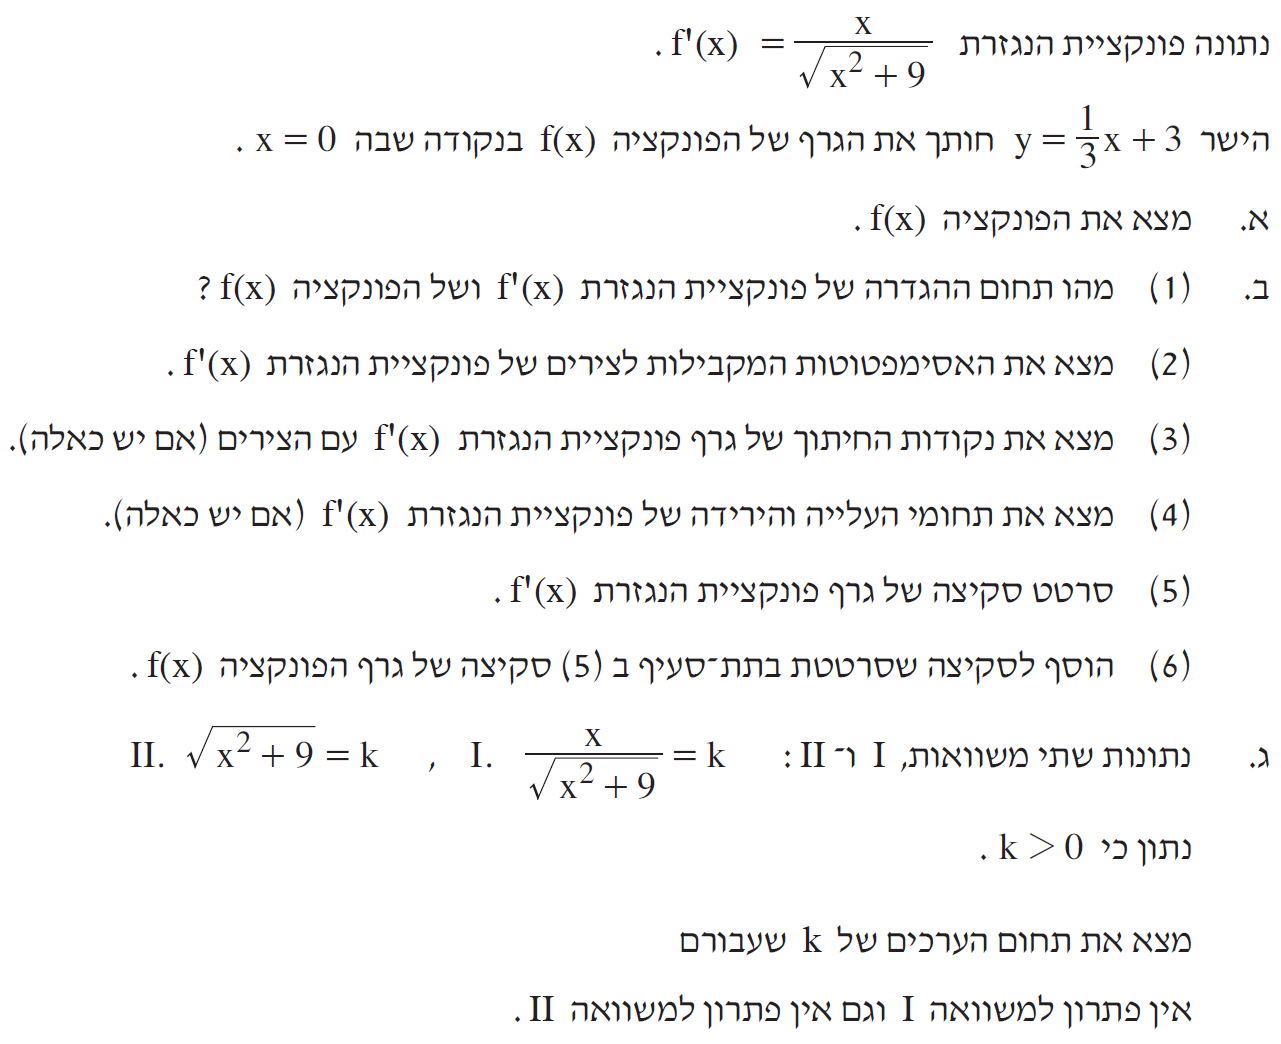
\includegraphics[width=.95\textwidth]{summer-2015b-7}
\end{center}

\vspace{-2ex}

\textbf{סעיף א}

\[
f(x)=\int f'(x) dx = \int \frac{1}{2}(x^2+9)^{-\frac{1}{2}}\cdot 2x\: dx = (x^2+9)^{\frac{1}{2}} +c\,.
\]
לפי הנתון,
$\sqrt{0^2+9}+c=3$,
ולכן
$c=0$
ו-%
$f(x) = \sqrt{x^2+9}$.

\textbf{סעיף ב}

$(1)$
$x^2+9$
חיובי עבור כל 
$x$
לכן
$f(x)$
ו-%
$f'(x)$
מוגדרות עבור כל
$x$.

$(2)$
$f'(x)$
מוגדרת עבור כל 
$x$
אז אין
\asms{}
אנכיות.

\[
\frac{\disfrac{x}{|x|}}{\sqrt{1+\disfrac{9}{x^2}}}\limit{\pm\infty}\pm 1\,,
\]
לכן 
$y=1$
היא 
\asm{}
אופקית כאשר
$x\rightarrow +\infty$,
ו-%
$y=-1$
היא
\asm{}
אופקית כאשר
$x\rightarrow -\infty$.


$(3)$
על ידי הצבה של
$x=0$
יש נקודת חיתוך ב-%
$(0,0)$.

המכנה חיובי לכן 
$y=0$
רק אם 
$x=0$
וכבר קיבלנו נקודת חיתוך זו.

\np

$(4)$
\[
f''(x)= \frac{1\cdot\sqrt{x^2+9}- x\cdot \disfrac{1}{2} \disfrac{1}{\sqrt{x^2+9}}\cdot 2x}{x^2+9}=\frac{9}{(x^2+9)\sqrt{x^2+9}}\,.
\]
הנגזרת השנייה תמיד חיובית ולכן הנגזרת הראשונה עולה בכל התחום.

\smallskip

$(5,6)$
ל-%
$f(x)$
נקודת מינימום ב-%
$(0,3)$.
מסעיף 
$(4)$
הנגזרת הראשונה עולה בכל התחום. הסימן של 
$f'(x)$
שלילית עבור ערכים שליליים של 
$x$
וחיובית עבור ערכים חיוביים.

לפי 
$(3)$
ל-%
$f'(x)$
יש נקודת חיתוך ב-%
$(0,0)$.
לפי 
$(2)$
יש 
\asms{}
ב-%
$\pm 1$
כאשר השאיפה היא ל-%
$1$
עבור 
$x\rightarrow +\infty$,
ול-%
$-1$
עבור 
$x\rightarrow -\infty$.

\begin{center}
\selectlanguage{english}
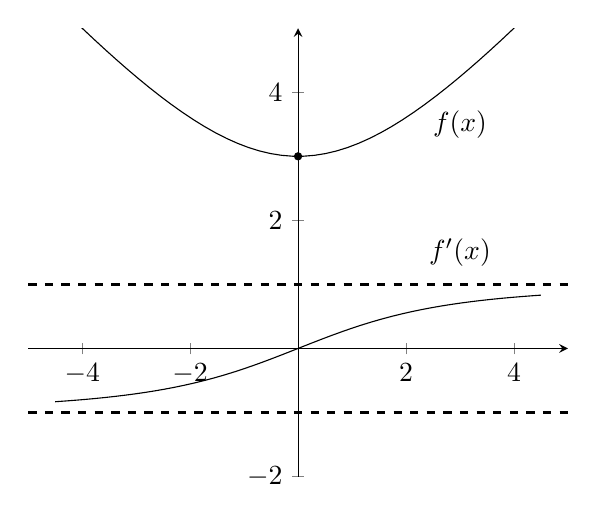
\begin{tikzpicture}%[scale=.8]
\begin{axis}[
    axis lines=center,
    xmin = -5,
    xmax = 5,
    ymin = -2,
    ymax = 5,
]
\addplot [
    domain=-5:5,
    samples=50, 
]
{sqrt(x^2+9)};
\addplot [
    domain=-4.5:4.5,
    samples=50, 
]
{(x)/(sqrt(x^2+9))};
\draw[dashed,thick] (axis cs:-5,1) -- (axis cs:5,1);
\draw[dashed,thick] (axis cs:-5,-1) -- (axis cs:5,-1);
\fill (axis cs:0,3) circle(1.5pt);
\node at (axis cs:3,3.5) {$f(x)$};
\node at (axis cs:3,1.5) {$f'(x)$};
\end{axis}
\end{tikzpicture}
\end{center}


\textbf{סעיף ג}

הערך הקטן ביותר של
$\sqrt{x^2+9}$
הוא
$3$,
ולכן אין פתרון למשוואה II כאשר
$0<k<3$.
זה ברור גם מהגרף כי
$(0,3)$
היא נקודת מינימום של
$f(x)$.

מהגרף של
$f'(x)$
ברור שאין פתרון למשוואה I כאשר 
$k\geq 1$.
אפשר גם בחישוב:
\erh{12pt}
\begin{equationarray*}{rcl}
\frac{x^2}{x^2+9}&=&k^2\\
x&=&\frac{3k}{\sqrt{1-k^2}}\,.
\end{equationarray*}
כדי שניתן להוציא שורש חייב להתקיים
$k<1$,
ולכן אין פתרון כאשר
$k\geq 1$.

שימו לב שהשאלה ביקשה את התחום בו אין פתרון ל-I 
\textbf{וגם}
ל-II. צירוף שתי התוצאות נותן שאין פתרון לשתי המשוואות כאשר
$1\leq k < 3$.

\np


%%%%%%%%%%%%%%%%%%%%%%%%%%%%%%%%%%%%%%%%%%%%%%%%%%%%%%%%%%%%%%%%%%%%%%

\section{קיץ תשע"ה מועד א}

\begin{center}
\selectlanguage{english}
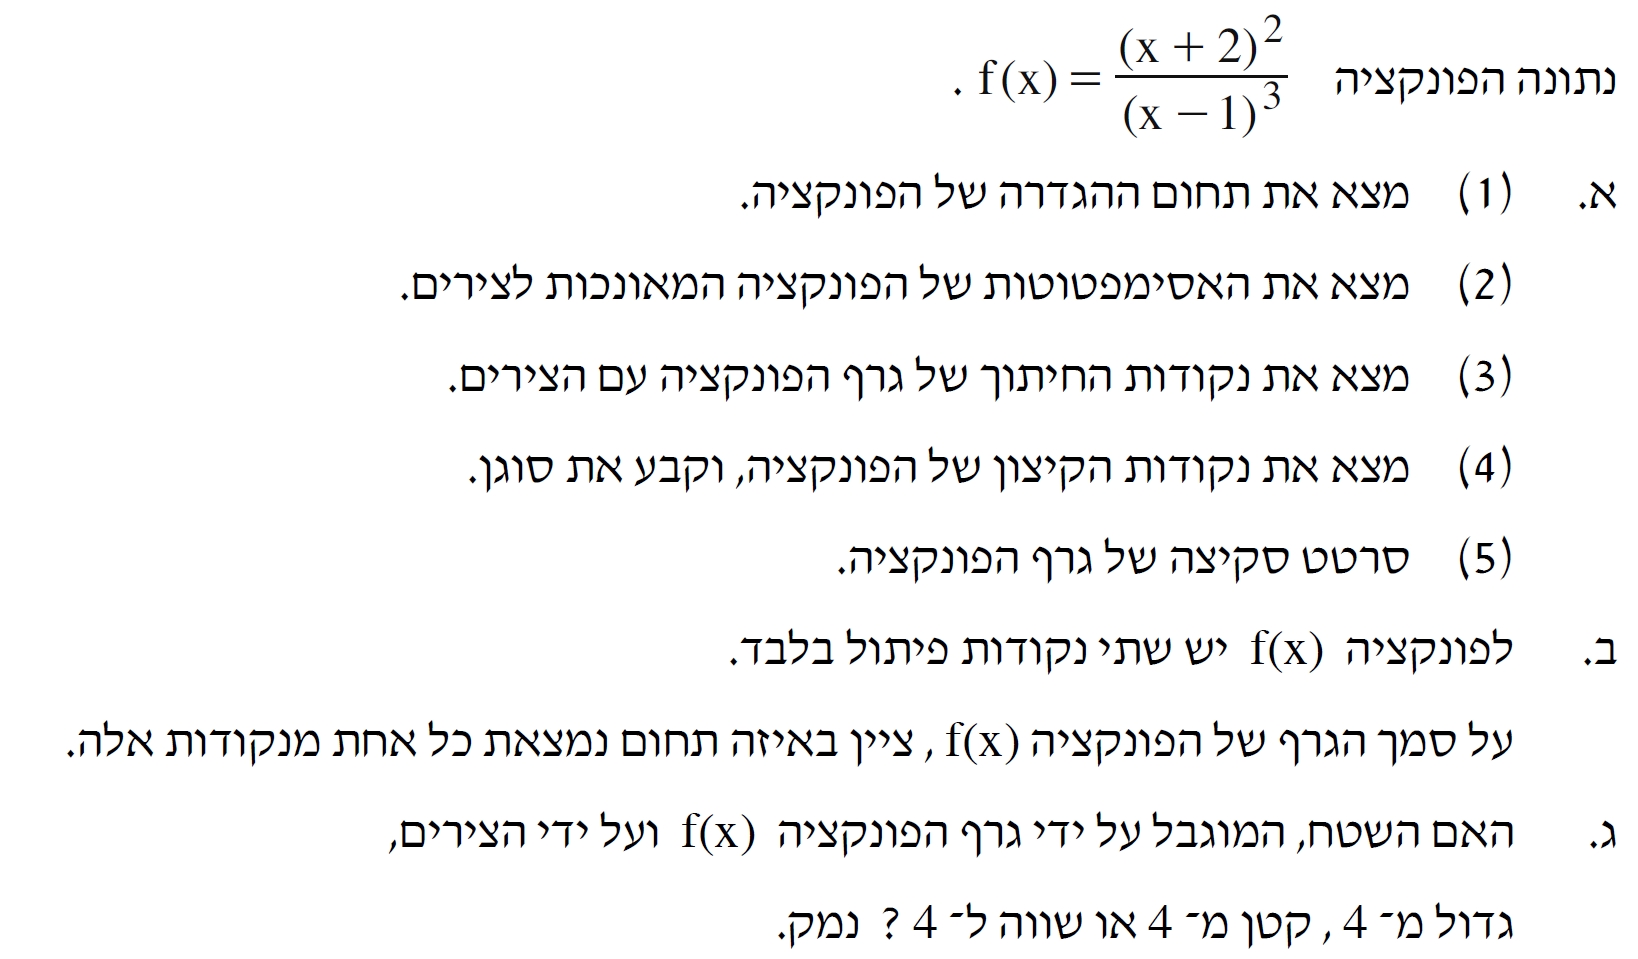
\includegraphics[width=.9\textwidth]{summer-2015a-7}
\end{center}

\vspace{-2ex}

\textbf{סעיף א}

$(1)$
הפונקציה לא מוגדרת כאשר המכנה מתאפס ב-%
$x=1$.
תחום ההגדרה הוא
$x\neq 1$.

$(2)$
כאשר
$x=1$
המכנה מתאפס אבל המונה לא מתאפס, לכן 
$x=1$
היא
\asm{}
אנכית.

\[
\disfrac{\disfrac{x^2}{x^3}+\disfrac{4x}{x^3}+\disfrac{4}{x^3}}
{\disfrac{x^3}{x^3}-\frac{3x^2}{x^3}+\frac{3x}{x^3}-\frac{1}{x^3}}
\limit{\pm\infty}0\,.
\]
הכנה שואף ל-%
$1$
והמונה שואף ל-%
$0$,
ולכן יש
\asm{}
אופקית ב-%
$y=0$.

$(3)$
כאשר 
$x=0$,
$y=\frac{4}{-1}=-4$.

כדי ש-%
$y=0$,
$(x+2)^2=0$,
$x=-2$
והמכנה לא מתאפס עבור
$x=-2$.

נקודות החיתוך הן
$(0,-4), (-2,0)$.

$(4)$
\[
f'(x)=\frac{2(x+2)(x-1)^3-(x+2)^2\cdot 3(x-1)^2}{(x-1)^6}=-\frac{(x+2)(x+8)}{(x-1)^6}\,.
\]
המכנה לא מתאפס בתחום ההגדרה, לכן נקודות הקיצון הן
$(-2,0), \left(-8,-\disfrac{4}{81}\right)$.

המכנה חיובי ולכן סימן הנגזרת השנייה שווה לסימן הנגזרת של המונה
$-2(x+5)$.

$-2(-2+5)<0$
ולכן
$(-2,0)$
היא מקסימום.

$-2(-8+5)>0$
ולכן
$\left(-8,-\disfrac{4}{81}\right)$
היא מינימום.

\np

$(5)$
לא ניתן לראות את כל המידע החשוב בגרף בקנה מידה אמיתי. הבאתי שני גרפים, אחד מימין לציר ה-%
$y$
מהראה את ה%
\asms{},
ואחד משמאל לציר ה-%
$y$
המראה את נקודות הקיצון.

\begin{center}
\begin{minipage}{.48\textwidth}
\selectlanguage{english}
\begin{tikzpicture}[scale=.8]
\begin{axis}[
    axis lines=center,
    xmin = -1,
    xmax = 5,
    ymin = -800,
    ymax = 400,
    ymajorticks=false,
]
\addplot [
    domain=-12:.8,
    samples=100, 
]
{(2*(x+2)^2)/((x-1)^3)};
\addplot [
    domain=1.2:8,
    samples=50, 
]
{((x+2)^2)/((x-1)^3)};
\draw[dashed,thick] (axis cs:1,-800) -- (axis cs:1,400);
\end{axis}
\end{tikzpicture}
\end{minipage}
\begin{minipage}{.48\textwidth}
\selectlanguage{english}
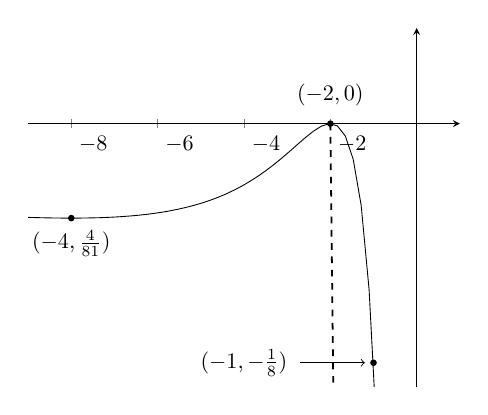
\begin{tikzpicture}[scale=.8]
\begin{axis}[
    axis lines=center,
    xmin = -9,
    xmax = 1,
    ymin = -5.5,
    ymax = 2,
    xticklabel style={anchor=north west},
    ymajorticks=false,
]
\addplot [
    domain=-9:0,
    samples=50, 
]
{(40*(x+2)^2)/((x-1)^3)};
\fill (axis cs: -2,0) circle(1.5pt);
\fill (axis cs: -8,-1.975) circle(1.5pt);
\node at (axis cs: -2,.6) {$(-2,0)$};
\node at (axis cs: -8,-2.5) {$(-4,\frac{4}{81})$};
\draw[thick,dashed] (axis cs:-2,0) -- (axis cs:0,-160);
\fill (axis cs: -1,-5) circle(1.5pt);
\node at (axis cs: -4,-5) {$(-1,-\frac{1}{8})$};
\draw[->] (axis cs:-2.7,-5) -- (axis cs:-1.2,-5);
\end{axis}
\end{tikzpicture}
\end{minipage}
\end{center}

\textbf{סעיף ב}

בין 
$-\infty$
ל-%
$-8$,
השיפוע יורד ואז עולה ויש נקודת פיתול. בין
$-8$
ל-%
$-2$
השיפוע עולה ואז יורד ויש נקודת פיתול.

\textbf{סעיף ג}

הקן בין 
$(-2,0)$
לבין
$(0,-4)$
תוחם משולש )ישר זווית( ששטחו
$\frac{1}{2}\cdot 2 \cdot 4=4$.
הגרף נמצאת מעל לקו לכן השטח שהוא תוחם פחות מ-%
$4$.

בגלל קנה המידה בתרשים קשה לראות שהגרף תמיד מעל לקו המקווקוו, אז נבדוק בחישוב. ב-%
$x=-1$,
$f(-1)=-\frac{1}{8}=-0.125$.
לפי משולשים דומים, 
$x=-1$
חוצה את הבסיס ולכן הנקודה על היתר של המשולש היא
$(-1,-2)$.
הגרף מעל לקו כי
$-0.125>-2$.



\np



%%%%%%%%%%%%%%%%%%%%%%%%%%%%%%%%%%%%%%%%%%%%%%%%%%%%%%%%%%%%%%%%%%%%%%

\section{חורף תשע"ה}

\begin{center}
\selectlanguage{english}
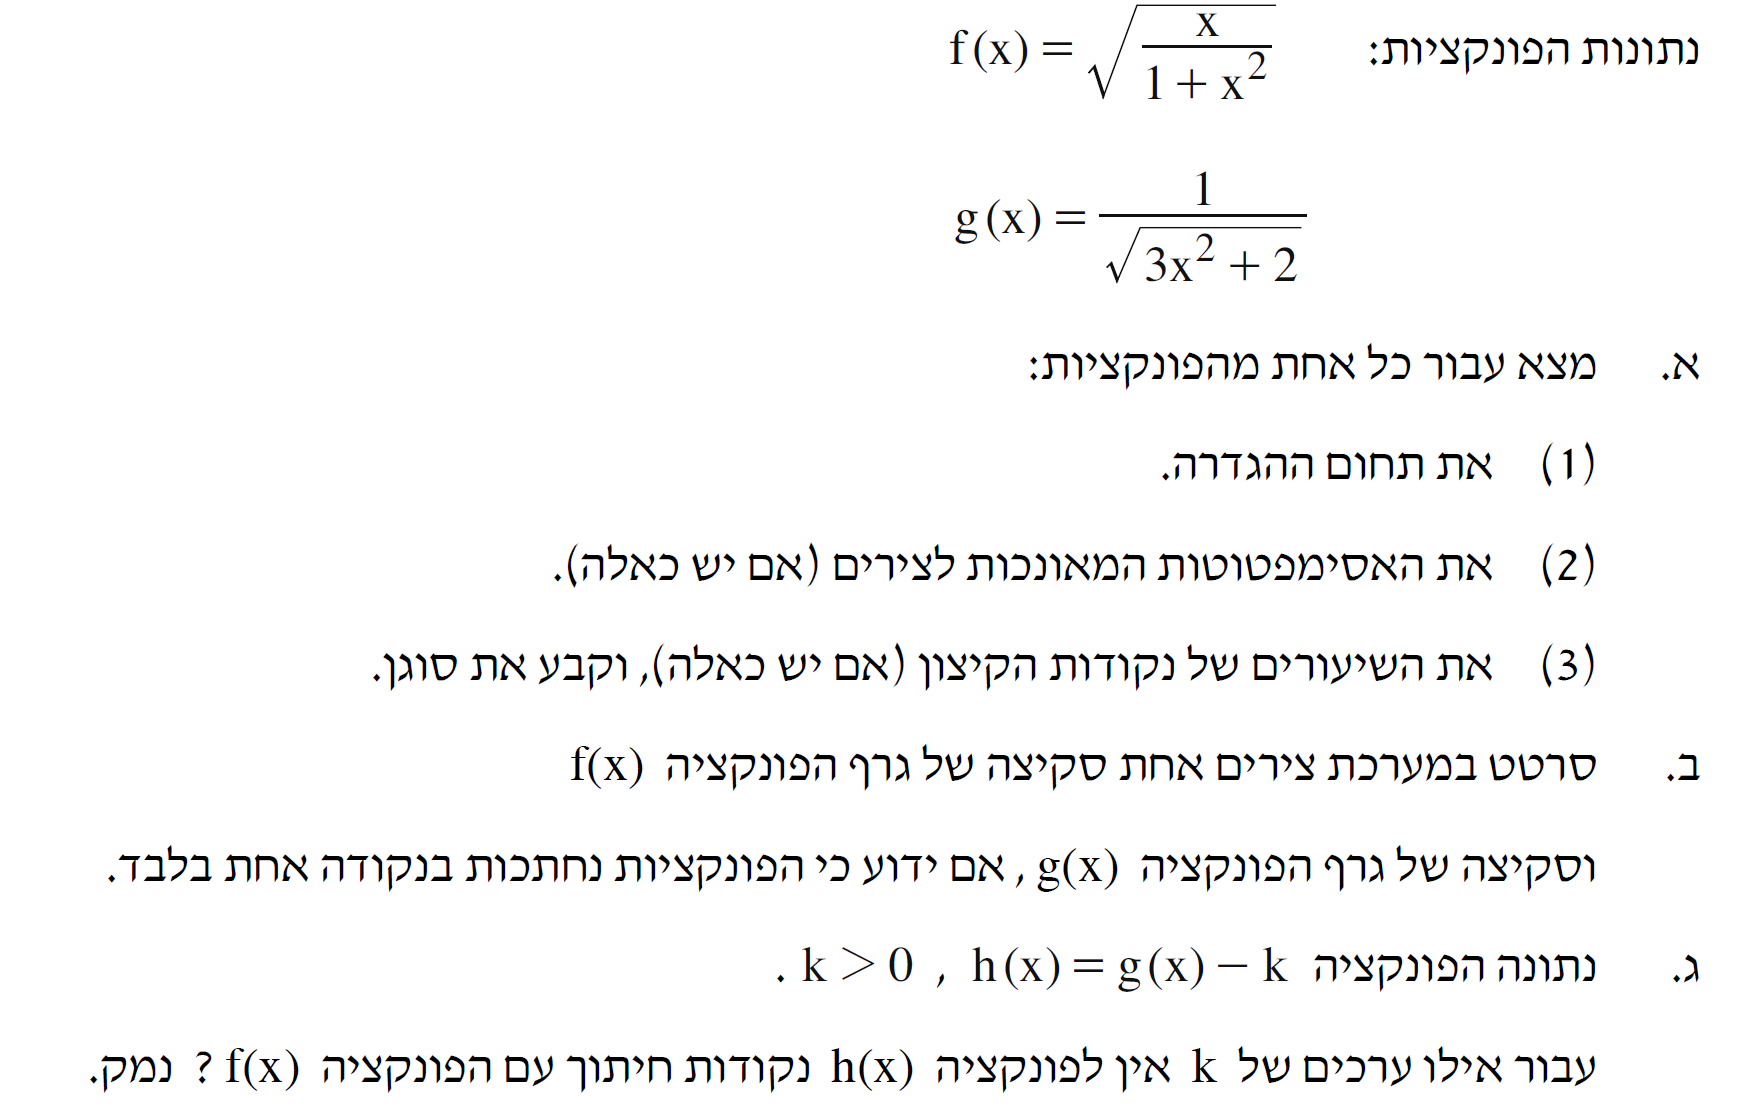
\includegraphics[width=\textwidth]{winter-2015-7}
\end{center}

\vspace{-2ex}

\textbf{סעיף א}

$(1)$
המכנה של שתי הפונקציות חיובי, ולכן 
$g(x)$
מוגדרת עבור כל
$x$.
$f(x)$
לא מוגדרת עבור
$x<0$
בגלל ה-%
$x$
במונה, כך שתחום ההגדרה הוא
$x\geq 0$.

$(2)$
אין 
\asms{}
אנכיות הפונקציות מוגדרת כל אחת בתחום שלה.
\[
\sqrt{\frac{\disfrac{x}{x^2}}{\disfrac{1}{x^2}+1}}\limit{+\infty} 0\,,
\]
ולכן
$y=0$
היא
\asm{}
אופקית.

כאשר
$x\limit{\pm\infty}$,
המכנה של
$g(x)$
שהוא חיובי שואף ל-%
$+\infty$,
ולכן
$y=0$
היא
\asm{}
אופקית.

$(3)$
עבור
$f(x)$:
\[
f'(x)= \frac{1}{2} \left(\frac{x}{1+x^2}\right)^{-\frac{1}{2}}\left(\frac{1\cdot(1+x^2)-x\cdot (2x)}{\disfrac{x}{1+x^2}}\right)=\frac{1}{2} \frac{1-x^2}{\left(\disfrac{x}{1+x^2}\right)^{\frac{3}{2}}}\,.
\]
המכנה חיובי והנגזרת מתאפסת כאשר המונה מתאפס
$x=\pm 1$.
$f(x)$
לא מוגדרת כאשר 
$x<0$
ונקודת הקיצון היחידה היא
$\left(1,\sqrt{\frac{1}{2}}\right)$.
הסימן של הנגזרת השנייה שווה לסימן של הנגזרת של המונה:
$\frac{1}{2}\cdot -2x$
שהיא שלילית עבור כל 
$x$
בתחום, ולכן נקודת הקיצון היא מקסימום.

\np

עבור
$g(x)$:
\[
g'(x)= -\frac{1}{2} \left(3x^2+2\right)^{-\frac{3}{2}}\cdot 6x\\
\]
המכנה חיובי לכן הנגזרת מתאפסת כאשר 
$x=0$.
נקודת הקיצון היא
$\left(0,\sqrt{\frac{1}{2}}\right)$.
הנגזרת של המונה היא
$-3<0$,
ונקדות הקיצון היא מקסימום.

\smallskip

\textbf{סעיף ב}

\vspace{-2ex}

\begin{center}
\selectlanguage{english}
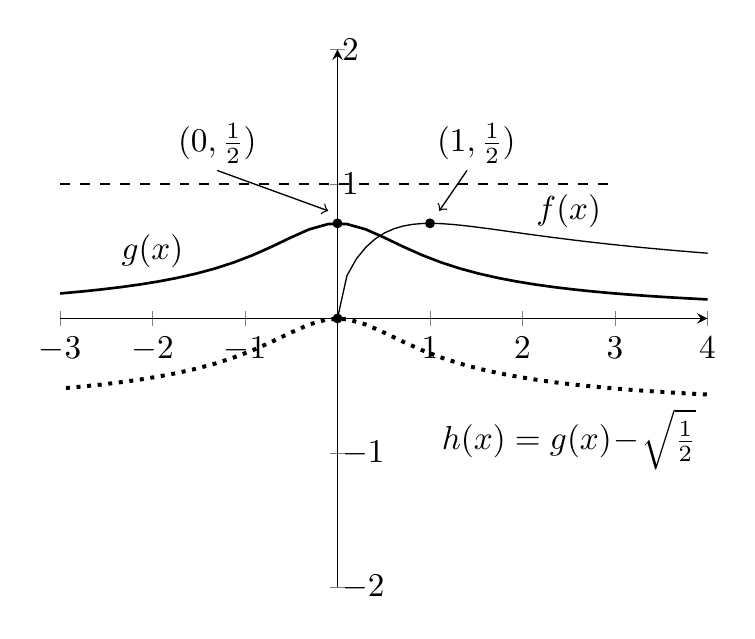
\begin{tikzpicture}[scale=1.2]
\begin{axis}[
    axis lines=center,
    xmin = -3,
    xmax = 4,
    ymin = -2,
    ymax = 2,
    yticklabel style={anchor=west,},
]
\addplot [
    domain=0:5, 
    samples=50, 
]
{sqrt((x)/(1+x^2))};
\addplot [
    domain=-5:5, 
    samples=50,
    thick, 
]
{(1)/(sqrt(3*x^2+2))};
\addplot [
    domain=-5:5, 
    samples=50,
    very thick, 
    dotted,
]
{(1)/(sqrt(3*x^2+2))-.707};
\draw[dashed,thick] (axis cs:-3,1) -- (axis cs:3,1);
\fill (axis cs: 0,.707) circle(1.5pt);
\fill (axis cs: 1,.707) circle(1.5pt);
\fill (axis cs: 0,0) circle(1.5pt);
\node at (axis cs: -2,.5) {$g(x)$};
\node at (axis cs: 2.5,.8) {$f(x)$};
\node at (axis cs: 2.5,-.9) {$h(x)=g(x)\!-\!\sqrt{\frac{1}{2}}$};
\node at (axis cs: -1.3,1.3) {$(0,\frac{1}{2})$};
\node at (axis cs: 1.5,1.3) {$(1,\frac{1}{2})$};
\draw[->] (axis cs: -1.3,1.1) -- (axis cs:-.1,.8); 
\draw[->] (axis cs: 1.4,1.1) -- (axis cs:1.1,.8); 
\end{axis}
\end{tikzpicture}
\end{center}

\vspace{-2ex}

ההערה "אם ידוע כי הפונקציות תחתכות בנקודה אחת בלבד" היתה לי די מוזרה, אבל לאחר מחשבה הבנתי שההערה באה למנוע אפשר של חיתוך כאשר
$x>1$
ושואף לאינסוף.

רציתי להשתכנע שאכן ההערה נכונה. כאשר משווים 
$f(x)=g(x)$
ומפשטים, מקבלים משוואה ממעלה שלישי:
\[
3x^3-x^2+2x-1=0\,.
\]
לא חיפשתי את הנוסחה )המסובכת( למציאת פתרונות למשוואות ממעלה שלישי, אבל לבסוף שמתי לב שאם
$x>1$
אז
$3x^3-x^2>0$
ו-%
$2x-1>0$,
ולכן לא יכול להיות פתרונות נוספים.

\textbf{סעיף ג}

הערך המינימלי של 
$f(x)$
הוא
$0$,
והערך המקסימלי של
$g(x)$
הוא
$\sqrt{\frac{1}{2}}$.
אם
$k>\sqrt{\frac{1}{2}}$
לא יהיו נקודות חיתוך בין שתי הפונקציות.

\np

%%%%%%%%%%%%%%%%%%%%%%%%%%%%%%%%%%%%%%%%%%%%%%%%%%%%%%%%%%%%%%%%%%%%%%

\section{קיץ תשע"ד מועד ב}

\begin{center}
\selectlanguage{english}
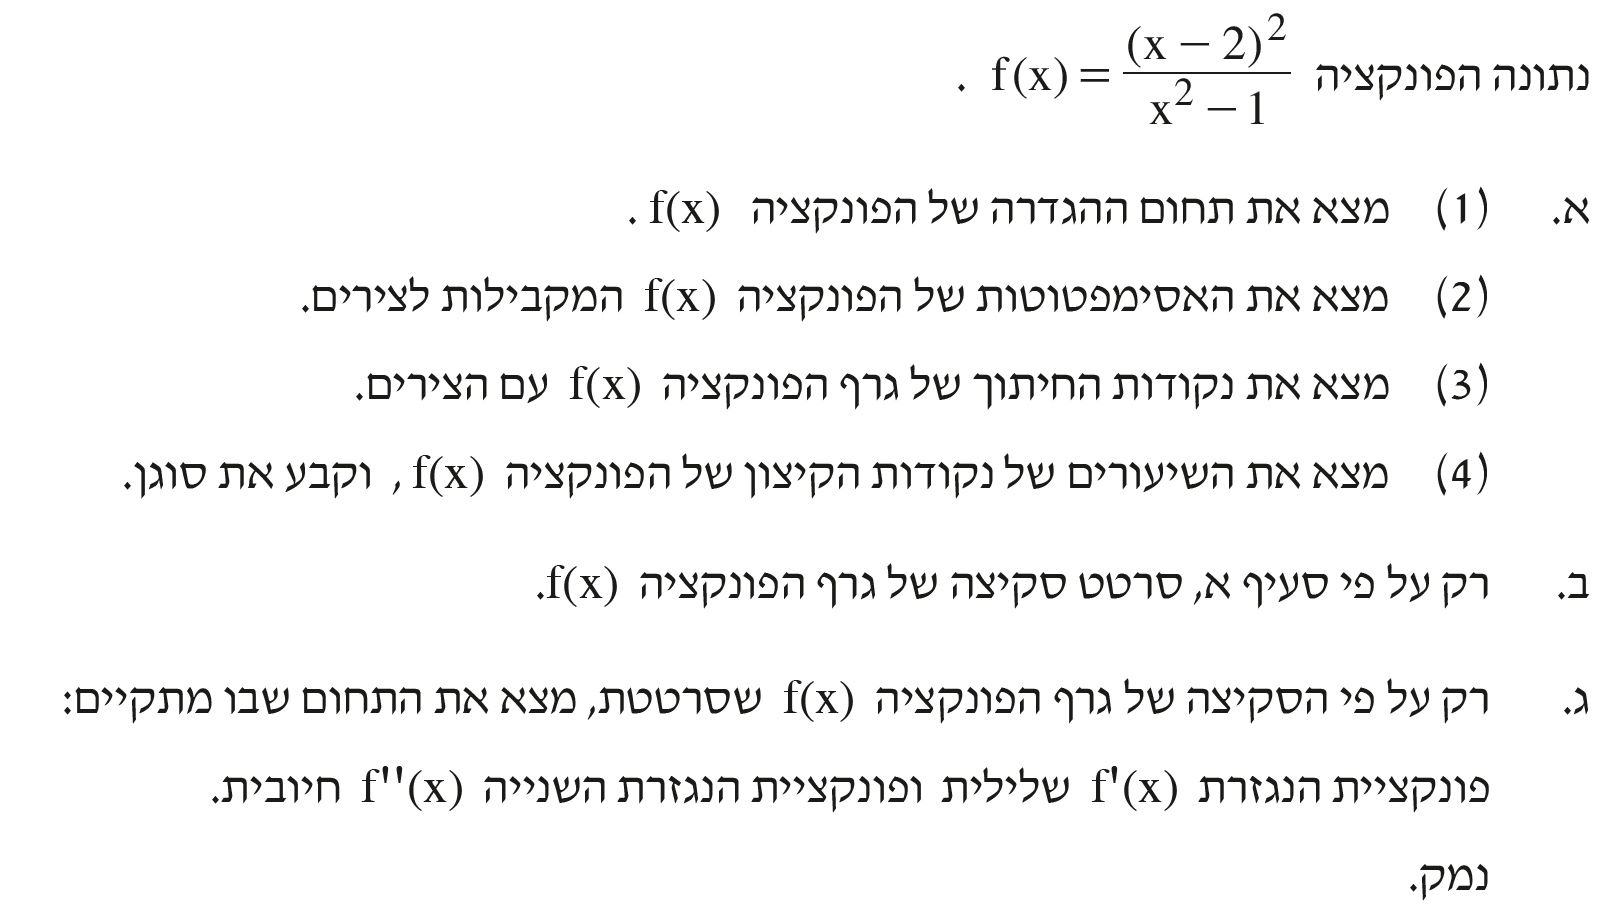
\includegraphics[width=.95\textwidth]{summer-2014b-7}
\end{center}

\vspace{-2ex}

\textbf{סעיף א}

$(1)$
הפונקציה לא מוגדרת כאשר המכנה מתאפס 
$x=\pm 1$.

$(2)$
ה%
\asms{}
האנכיות הן במקומות שהפונקציה לא מוגדרת
$x=\pm 1$.

חישוב ה%
\asm{}
האופקית
$y=1$:
\[
\frac{1-\disfrac{4}{x}+\disfrac{4}{x^2}}{1-\disfrac{1}{x^2}}\limit{\pm\infty}\disfrac{1}{1}=1\,.
\]
$(3)$
כאשר
$x=0$,
$y=-4$.

כאשר 
$x=2$
המונה מתאפס והמכנה לא מתאפס.

נקודות החיתוך הן
$(2,0), (0,-4)$.

$(4)$
חישוב הנגזרת הראשונה:
\[
f'(x)=\frac{2(x-2)(x^2-1)-(x-2)^2\cdot 2x}{(x^2-1)^2}=\frac{2(2x^2-5x+2)}{(x^2-1)^2}=(2x-1)(x-2)\,.
\]
המכנה חיובי בתחום ההגדרה ולכן נקודות הקיצון נמצאות ב-%
$x=2,x=\frac{1}{2}$.

המכנה חיובי לכן סימן הנגזרת השנייה שווה לסימן הנגזרת של המונה:
$2(4x-5)$.
ביטוי זה חיובי עבור
$x=2$,
ושלילי עבור
$x=\frac{1}{2}$.
נקודות הקיצון הן:
\[
(2,0)\quad \textrm{\R{מינימום}},\quad\quad \left(\frac{1}{2},-3\right)\quad \textrm{\R{מקסימום}}\,.
\]

\np

\textbf{סעיף ב}

חישבנו את ה%
\asms{},
נקודות החיתוך עם הצירים וונקודות הקיצון. מידע זה מספיק לצייר תרשים עבור 
$x>-1$.
עבור
$x<-1$
נבדוק אם הגרף מעל ל%
\asm{}
האופקית או מתחתיה.
$f(-2)=\frac{16}{3}>1$
ולכן הגרף מעל ל%
\asm{}.

\begin{center}
\selectlanguage{english}
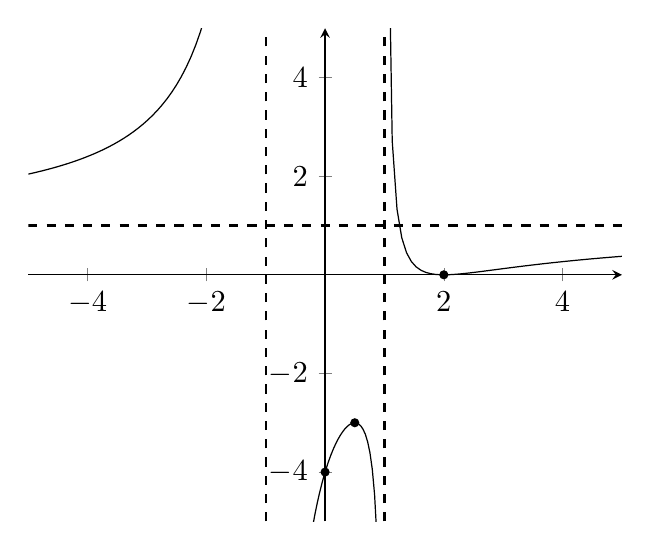
\begin{tikzpicture}[scale=1.1]
\begin{axis}[
    axis lines=center,
    xmin = -5,
    xmax = 5,
    ymin = -5,
    ymax = 5,
]
\addplot [
    domain=-5:-1.05, 
    samples=50, 
]
{(x-2)^2)/(x^2-1)};
\addplot [
    domain=-.95:.95, 
    samples=50, 
]
{(x-2)^2)/(x^2-1)};
\addplot [
    domain=1.05:5, 
    samples=50, 
]
{(x-2)^2)/(x^2-1)};
\draw[dashed,thick] (axis cs:-1,-5) -- (axis cs:-1,5);
\draw[dashed,thick] (axis cs:1,-5) -- (axis cs:1,5);
\draw[dashed,thick] (axis cs:-5,1) -- (axis cs:5,1);
\fill (axis cs: 0,-4) circle(1.5pt);
\fill (axis cs: .5,-3) circle(1.5pt);
\fill (axis cs: 2,0) circle(1.5pt);
\end{axis}
\end{tikzpicture}
\end{center}


\textbf{סעיף ג}

כדי שהנגזרת הראשונה תהיה שלילית, הפונקציה חייבת לרדת: 
\[
\frac{1}{2}< x < 1, \quad 1<x<2\,.
\]
כדי שהנגזרת השנייה תהיה חיובית, הנגזרת הראשונה חייבת לעלות:
\[
x<-1,\quad  1<x<x_1\,,
\]
כאשר 
$x_1$
היא נקודת הפיתול אי-שם מימין ל-%
$x=2$.

החיתוך בין שני התחומים הוא
$1<x<2$.

\np


%%%%%%%%%%%%%%%%%%%%%%%%%%%%%%%%%%%%%%%%%%%%%%%%%%%%%%%%%%%%%%%%%%%%%%

\section{קיץ תשע"ד מועד א}

\begin{center}
\selectlanguage{english}
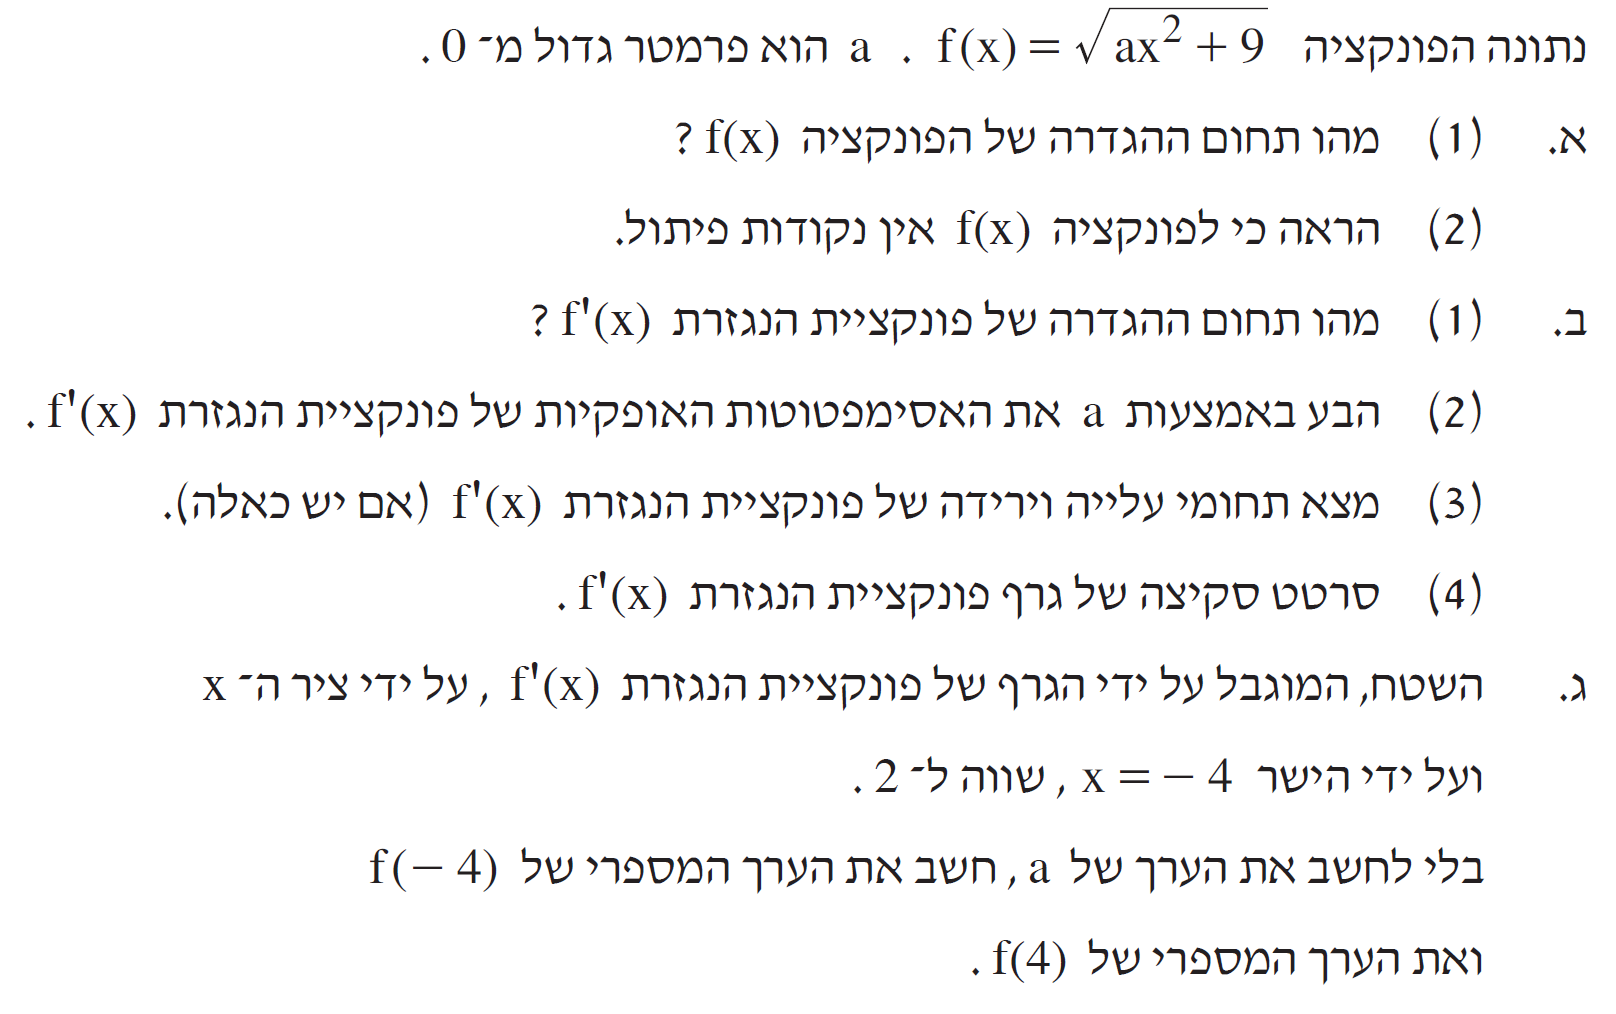
\includegraphics[width=.9\textwidth]{summer-2014a-7}
\end{center}

\vspace{-2ex}

\textbf{סעיף א}

$(1)$
הפונקציה לא מוגדר כאשר 
$ax^2+9\leq 0$.
נתון ש-%
$a>0$
אז הביטוי תמיד גדול מאפס, והפונקציה מוגדרת עבור כל 
$x$.

$(2)$
נחשב את הנגזרת הראשונה והנגזרת השנייה:
\erh{2pt}
\begin{equationarray*}{rcl}
f'(x)&=&\frac{1}{2}(ax^2+9)^{-\frac{1}{2}}\cdot 2ax= \frac{ax}{\sqrt{ax^2+9}}\\
&&\\
f''(x)&=&\frac{a\sqrt{ax^2+9}-ax\cdot \disfrac{ax}{\sqrt{ax^2+9}}}{ax^2+9}\\
&&\\
&=&\frac{9a}{(ax^2+9)\sqrt{ax^2+9}}\,.
\end{equationarray*}
)א( הנגזרת השנייה מוגדרת לכל 
$x$,
ו-)ב( גם המונה וגם המכנה חיוביים, ולכן הנגזרת השנייה לא מתאפסת. המסקנה היא שאין נקודות פיתול.

\textbf{סעיף ב}

$(1)$
$f'(x)$
מוגדרת כאשר 
$ax^2+9>0$,
ולכן היא מוגדרת לכל 
$x$
בדיוק כמו
$f(x)$.


$(2)$
יש
\asms{}
אופקיות ב-%
$\pm\sqrt{a}$:
\[
f'(x)=\disfrac{\disfrac{ax}{|x|}}{\sqrt{a+\disfrac{9}{x^2}}}\limit{\pm\infty} \pm\sqrt{a}\,.
\]

\np

$(3)$
ראינו בסעיף א שהנגזרת השנייה תמיד חיובית ולכן הנגזרת הראשנוה תמיד עולה.

$(4)$
נשתמש במידע: 
$f'(0)=0$,
יש
\asms{}
אופקיות ב-%
$\pm\sqrt{a}$,
הנגזרת תמיד עולה:
\begin{center}
\selectlanguage{english}
\begin{tikzpicture}[scale=1]
\begin{axis}[
    axis lines=center,
    xmin = -4.2,
    xmax = 4,
    ymin = -2,
    ymax = 2,
    yticklabel style = {anchor=north east},
    xticklabel style = {anchor=north east},
]
\addplot [
    domain=-4:4, 
    samples=50, 
]
{x/sqrt(x^2+9)};
\draw[dashed,thick] (axis cs:-4,1) -- (axis cs:4,1);
\draw[dashed,thick] (axis cs:-4,-1) -- (axis cs:4,-1);
\draw[dashed,ultra thick] (axis cs:-4,0) -- (axis cs:-4,-.8);
\node at (axis cs:3.3,-1.3) {$-\sqrt{a}$};
\node at (axis cs:3.3,1.3) {$\sqrt{a}$};
\end{axis}
\end{tikzpicture}
\end{center}

\textbf{סעיף ג}

האינטגרל של הנגזרת של פונקציה הוא הפונקציה עצמה.
\[
\int_{-4}^{0} 0-f'(x)dx = -\int_{-4}^{0}f'(x)dx = \left.-f(x)\rule{0pt}{12pt}\right|_{-4}^{0} = -f(0) + f(-4)\,.
\]
קל לחשב ש-%
$f(0)=\sqrt{9}=3$
ו-%
$f(-4)=\sqrt{16a+9}$.
הפיתוי הוא לחשב את הערך של 
$a$
אבל השאלה דורשת את הערך של
$f(-4)$
בלי לחשב את הערך של
$a$.
החישוב אפילו קל יותר:
\begin{eqnarray*}
-f(0)+f(-4)&=&2\\
f(-4)&=&2+f(0)=2+3=5\,.
\end{eqnarray*}
הפונקציה זוגית, לכן
$f(4)=f(-4)=5$.

מי שמעוניין יכול לחשב את ערכו של 
$a$:
\begin{eqnarray*}
\sqrt{16a+9}&=&2+3\\
a&=&1\,.
\end{eqnarray*}


\np

%%%%%%%%%%%%%%%%%%%%%%%%%%%%%%%%%%%%%%%%%%%%%%%%%%%%%%%%%%%%%%%%%%%%%%

\section{חורף תשע"ד}

\begin{center}
\selectlanguage{english}
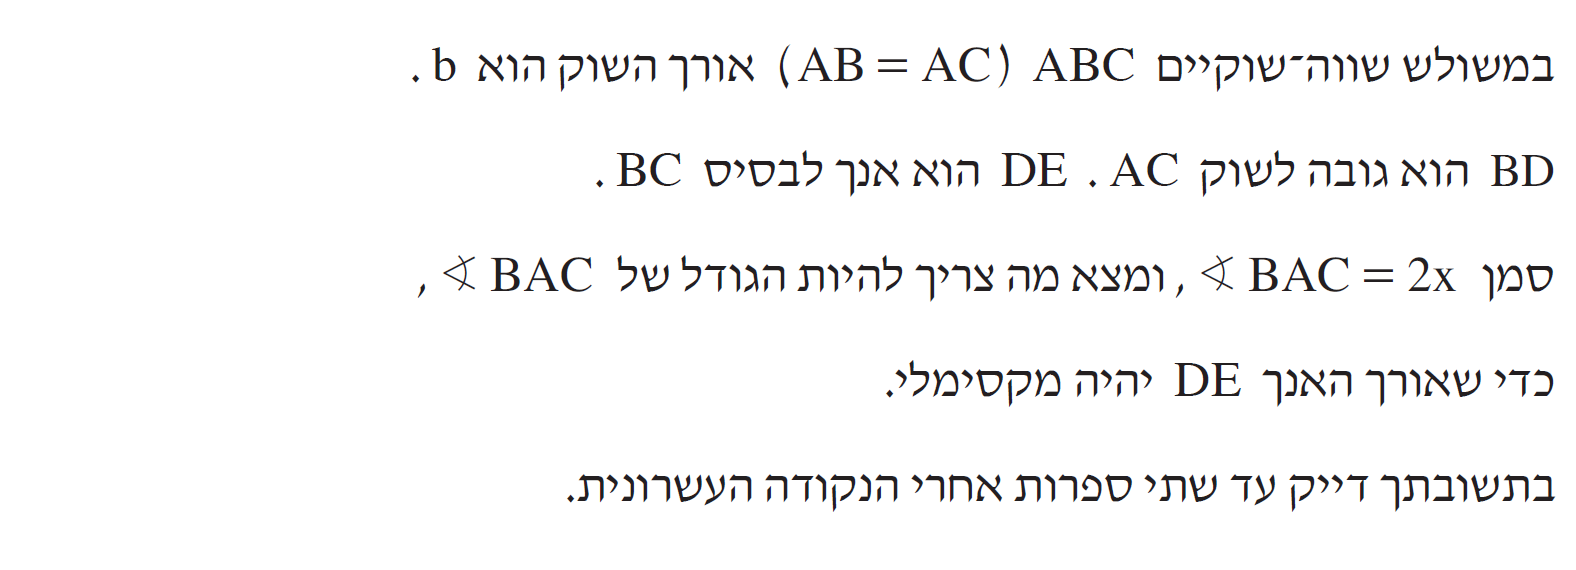
\includegraphics[width=.9\textwidth]{winter-2014-8}
\end{center}

\vspace{-4ex}

\textbf{בבחינה זו היו שלוש שאלות בפרק השני לכן מספר השאלה הוא 
$8$
ולא 
$7$.}

\begin{center}
\selectlanguage{english}
\begin{tikzpicture}%[scale=.7]
\coordinate (A) at (0,0);
\draw[thick] (A) -- node[left] {$b$} (-117.5:6) coordinate (B);
\draw[thick,name path=bc] (A) -- (-62.5:6) coordinate (C);
\draw[thick] (B) -- (C);
\draw[thick] (B) -- node[above] {$d$} ($(A)!(B)!(C)$) coordinate (D);
\draw[thick] (D) -- node[left] {$e$} ($(B)!(D)!(C)$) coordinate (E);
\fill (B) node[below] {$B$} node[above right,xshift=18pt] {$x$} circle(1.5pt);
\fill (A) node[above] {$A$} node[below,yshift=-12pt] {$2x$} circle(1.5pt);
\fill (C) node[below right] {$C$} node[above right] {$90-x$} circle(1.5pt);
\draw[<-,thick] ($(C)+(-12pt,8pt)$)-- +(14pt,0);
\fill (D) node[right] {$D$} circle(1.5pt);
\fill (E) node[below] {$E$} circle(1.5pt);
\draw[thick,rotate=90] (E) rectangle +(7pt,7pt);
\draw[thick,rotate=117.5] (D) rectangle +(7pt,7pt);
\end{tikzpicture}
\end{center}

נצדיק את סימון הזוויות בתרשים. cמשולש שווה-שוקיים זוויות הבסיס שוות והסכום כל הזוויות במשולש שווה
$180$:
\[
\angle ACB=\angle ABC=\frac{180-2x}{2}=90-x\,.
\]
במשולש ישר-זווית
$\triangle BDC$,
$\angle DBC=90-(90-x)=x$.

במבט ראשון נראה שאפשר למצוא את הערך המקסימלי של
$DE=e$
על ידי מציאת הנגזרת 
$e'=(d \sin x)' = d (\sin x)'=0$.
אבל זה לא נכון כי
$d$
איננה קבוע ולכן אי אפשר להוציא אותו מהנגזרת. נתון ש-%
$b$
קבוע, כך שעלינו למצוא ביטוי מהצורה
$e=b \cdot f(x)$.

את החישוב נבצע בשני שלבים, תחילה נבטא את 
$e$
כפוקציה של
$x,d$,
ואח"כ נבטא את
$d$
כפונקציה של
$x,b$.
אפשר להשתמש בחוק הסינוסים, אבל פשוט יותר להשתמש בהגדרת הפונקציות הטריגונמטריות במשלושים ישר-זווית
$\triangle BED,\triangle BDA$:
\erh{1pt}
\begin{equationarray*}{rcl}
e&=&d\sin x\\
d&=&b\sin 2x\\
e&=&(b\sin 2x)\sin x\\
&=&b(2\sin x \cos x)\sin x=2b\sin^2 x\cos x
\end{equationarray*}
\np
\erh{1pt}
\begin{equationarray*}{rcl}
e'&=&2b(2\sin x \cos x\cos x + \sin^2 x \cdot(-\sin x))\\
&=&2b\sin x(2\cos^2 x-\sin^2 x)=0\,.
\end{equationarray*}
הנגזרת מתאפסת אם 
$\sin x = 0$
שלא ייתכן, כי
$x=0,x=180$
אינם יכולים להיות זוויות במשולש. הנגזרת גם מתאפסת אם:
\erh{6pt}
\begin{equationarray*}{rcl}
2\cos^2 x-\sin^2 x&=&0\\
\left(\frac{\sin x}{\cos x}\right)^2 &=& 2\\
\tan x &=& \pm \sqrt{2}\\
x&=&54.74,\; 125.26\,.
\end{equationarray*}
אבל 
$\angle BAC=2x$
כך ש-%
$x=54.74$
הוא הפתרון האפשרי היחיד.

השאלה מבקשת את ערכו של הזוויות
$\angle BAC=2x=109.47$.

\npchap
